\chapter{IMPLEMENTASI DAN PENGUJIAN}
\vspace{1em}
\section{Implementasi Sistem}
\subsection{Data \textit{Preprocessing}}
Pada tahap ini, proses \textit{data preprocessing} dilakukan untuk menyiapkan data pose 3D yang akan digunakan dalam pelatihan dan evaluasi model DeciWatch. Dataset yang digunakan merupakan dataset AIST++ yang menyediakan anotasi gerakan tari dalam format koordinat 3D, namun karena keterbatasan akses terhadap data video asli, proses deteksi pose awal dilakukan menggunakan model SPIN (\textit{SMPLify-X In the Loop}) yang memiliki struktur skeleton yang sama.

Model SPIN digunakan untuk mengekstraksi data pose 3D dari video tari yang tersedia dalam dataset AIST++. Hasil prediksi pose 3D dari SPIN kemudian dipasangkan dengan data \textit{ground truth} yang tersedia untuk keperluan pelatihan dan evaluasi model DeciWatch. Pasangan data ini terdiri dari dua bagian: data input berupa hasil estimasi pose dari SPIN, dan data target berupa anotasi pose 3D asli dari dataset AIST++ yang tersedia secara terbatas.

Setiap data pose 3D disimpan dalam format {.npz} yang berisi beberapa array utama. Struktur file {.npz} ini dijelaskan sebagai berikut:

Struktur data dalam file {.npz} yang digunakan pada sistem ini memiliki beberapa \textit{key} utama yang berisi informasi penting terkait pose 3D manusia untuk setiap sekuens gerakan. Setiap file menyimpan satu sekuens gerakan yang terdiri dari sejumlah frame, dengan format array sebagai berikut:

\begin{itemize}
    \item {\textit{imgname}} : Array berisi nama file atau jalur gambar dari frame-frame dalam sekuens. Tipe datanya adalah {numpy.ndarray} satu dimensi, dengan jumlah elemen sesuai panjang sekuens. Setiap elemen berupa string yang merepresentasikan nama atau jalur gambar dari masing-masing frame.
    
    \item {\textit{pose}} : Array dua dimensi dengan bentuk {(N, 72)}, di mana {N} adalah jumlah frame dalam sekuens. Setiap baris mewakili rotasi 24 sendi tubuh manusia dalam format axis-angle (masing-masing 3 dimensi, total 72). Data ini digunakan sebagai representasi postur tubuh untuk setiap frame.
    
    \item {\textit{shape}} : Array dua dimensi dengan bentuk {(N, 10)}, yang merepresentasikan parameter bentuk tubuh manusia dalam model SMPL. Nilai-nilai ini menggambarkan variasi bentuk tubuh dan tetap konstan sepanjang sekuens dalam kebanyakan kasus.
    
    \item {\textit{joints\_3d}} : Array dua dimensi dengan bentuk {(N, 3)}, yang menyimpan koordinat 3D dari titik pusat tubuh atau \textit{root joint} pada setiap frame. Koordinat ini digunakan sebagai referensi posisi global dalam ruang 3D.
    
    \item {\textit{camera}} : Array dua dimensi yang menyimpan parameter kamera per frame. Parameter ini digunakan dalam proses transformasi koordinat dari ruang kamera ke ruang dunia, serta untuk kebutuhan rendering ulang atau evaluasi terhadap data hasil prediksi.
\end{itemize}

Struktur ini berlaku untuk seluruh file {.npz} baik pada data pelatihan maupun validasi. Fleksibilitas format ini memungkinkan pemrosesan dan pelatihan model temporal seperti DeciWatch secara efisien dan modular berdasarkan sekuens per gerakan.

Dataset yang digunakan terdiri dari dua bagian utama, yaitu data pelatihan (\textit{train}) dan data validasi (\textit{val}). Pada bagian \textit{train}, terdapat sebanyak 7.292 sekuens gerakan dengan total 5.916.474 frame. Sementara itu, bagian \textit{val} terdiri dari 3.840 sekuens dengan total 2.882.640 frame. Rata-rata panjang setiap sekuens berkisar antara 300 hingga 600 frame, bergantung pada durasi dan kompleksitas gerakan dalam video.

Setiap sekuens menyimpan data dalam format {.npz}, yang berisi atribut seperti {pose}, {shape}, {joints\_3d}, dan {camera}. Struktur ini memungkinkan pengolahan data secara terpisah per sekuens, sekaligus memudahkan pelatihan model berbasis waktu seperti DeciWatch yang membutuhkan urutan frame yang berurutan dan konsisten. Dengan struktur yang terorganisir dan skala data yang besar, model dapat dilatih untuk mengenali pola gerakan manusia secara lebih akurat dan stabil dari waktu ke waktu.

Jumlah frame yang besar dan cakupan gerakan yang beragam dalam dataset ini memberikan fondasi yang kuat bagi model DeciWatch untuk belajar pola gerakan manusia secara kompleks dan merepresentasikannya secara halus dalam prediksi pose 3D.

\subsection{Inisialisasi Dataset dan \textit{DataLoader}}

Sebelum proses pelatihan dimulai, sistem terlebih dahulu memuat data pelatihan dan data uji dengan memanfaatkan kelas dataset yang telah disesuaikan dengan konfigurasi yang ditentukan. Proses ini dilakukan dengan memanggil fungsi \textit{dataset\_class} dan memberikan parameter seperti nama estimator (dalam hal ini menggunakan SPIN), jenis representasi tubuh (3D), serta bagian data yaitu \textit{train} atau \textit{test}. Pemanggilan ini akan menghasilkan dua objek yaitu \textit{train\_dataset} dan \textit{test\_dataset}.

Selanjutnya, kedua objek dataset tersebut dibungkus ke dalam \textit{DataLoader} dari PyTorch untuk memfasilitasi pemrosesan data dalam bentuk mini-batch selama proses pelatihan dan evaluasi model. Untuk data pelatihan digunakan ukuran batch sebesar 512 dan opsi \textit{shuffle} diaktifkan agar data tersaji secara acak pada setiap epoch. Sementara itu, pada data pengujian digunakan batch size 1 tanpa \textit{shuffle}, agar urutan data tetap terjaga selama proses evaluasi.

\begin{lstlisting}[style=plainbox, caption={Inisialisasi \textit{dataset} dan \textit{DataLoader} untuk pelatihan dan pengujian}, label={lst:dataloader}]
train_dataset = dataset_class(
                    dataset_name='aist',
                    estimator='spin',
                    return_type='3D',
                    sample_interval=5,
                    smpl_model_dir="data/smpl/",
                    phase='train'
                )

test_dataset = dataset_class(
                    dataset_name='aist',
                    estimator='spin',
                    return_type='3D',
                    sample_interval=5,
                    smpl_model_dir="data/smpl/",
                    phase='test'
                )

train_loader = DataLoader(
                    dataset=train_dataset,
                    batch_size=512,
                    shuffle=True,
                    num_workers=4,
                    pin_memory=True,
                    worker_init_fn=worker_init_fn
                )

test_loader = DataLoader(
                    dataset=test_dataset,
                    batch_size=1,
                    shuffle=False,
                    num_workers=4,
                    pin_memory=True,
                    worker_init_fn=worker_init_fn
                )

\end{lstlisting}

Penggunaan \textit{DataLoader} ini sangat penting untuk mengoptimalkan performa proses pelatihan model, terutama dalam hal efisiensi pemuatan data dari penyimpanan ke memori. Pengaturan seperti jumlah \textit{worker} dan aktivasi \textit{pin memory} membantu meningkatkan kecepatan transfer data antar proses dan perangkat GPU.


\subsection{Pembuatan Model}

Pada tahap ini dilakukan perancangan dan konfigurasi arsitektur model untuk menyempurnakan prediksi pose 3D secara temporal. Model yang digunakan adalah DeciWatch, yaitu model prediktif berbasis \textit{transformer encoder-decoder} yang dirancang untuk memproses urutan pose manusia dan menghasilkan prediksi yang lebih halus dan konsisten antar frame.

\begin{lstlisting}[style=plainbox, caption={Potongan isi file {config.yaml}}, captionpos=t, label={lst:config_yaml}]
MODEL:
    TYPE: network
    ENCODER_TRANSFORMER_BLOCK: 5
    ENCODER_EMBEDDING_DIMENSION: 128
    ENCODER_HEAD: 4
    ENCODER_RESIDUAL: true
    DECODER_TRANSFORMER_BLOCK: 6
    DECODER_EMBEDDING_DIMENSION: 128
    DECODER_HEAD: 4
    DECODER_RESIDUAL: true
    DECODER_TOKEN_WINDOW: 5
    SLIDE_WINDOW: true
    SLIDE_WINDOW_SIZE: 51
    SLIDE_WINDOW_Q: 10
\end{lstlisting}

Arsitektur model terdiri dari \textit{transformer encoder-decoder}, dengan konfigurasi sebagai berikut:

\begin{itemize}
    \item Encoder terdiri dari 5 blok transformer, dimensi embedding 128, 4 \textit{attention head}, dengan koneksi residual.
    \item Decoder terdiri dari 6 blok transformer, embedding 128, dengan token window berukuran 5.
    \item Pendekatan \textit{sliding window} digunakan untuk proses input sekuens dengan ukuran jendela 51 frame dan langkah pergeseran 10.
    \item Sampling frame dilakukan setiap 5 frame secara seragam.
\end{itemize}

Dataset yang digunakan adalah AIST++ dengan representasi tubuh 3D, menggunakan 14 titik sendi utama tanpa aktivasi SMPL.

Model diimplementasikan dengan PyTorch menggunakan kelas {DeciWatch} yang diturunkan dari {nn.Module}, seperti pada kode berikut:

\begin{lstlisting}[style=plainbox, caption={Model {DeciWatch}},captionpos=t, label={lst:deciwatch_model}]
model = DeciWatch(input_dim=train_dataset.input_dimension,
                  sample_interval=5,
                  encoder_hidden_dim=128,
                  decoder_hidden_dim=128,
                  dropout=0.1,
                  nheads=4,
                  dim_feedforward=256,
                  enc_layers=5,
                  dec_layers=6,
                  activation="leaky_relu",
                  pre_norm=True,
                  recovernet_interJ_method="linear",
                  recovernet_mode="transformer").to('cuda')
\end{lstlisting}


Inisialisasi ini memanfaatkan nilai \textit{input dimension} dari dataset pelatihan untuk menentukan jumlah fitur per frame yang akan diproses oleh model. Dengan parameter yang fleksibel dan bersifat modular, sistem ini memungkinkan penyesuaian cepat terhadap jenis data, panjang sekuens, atau kompleksitas gerakan yang berbeda pada skenario pelatihan lain di masa mendatang.

Setelah model berhasil diinisialisasi, langkah berikutnya adalah mendefinisikan fungsi loss dan algoritma optimisasi yang akan digunakan selama proses pelatihan. Pada sistem ini, digunakan kelas \textit{DeciWatchLoss} yang dirancang khusus untuk menghitung selisih antara hasil prediksi model dengan data \textit{ground truth} dalam bentuk pose 3D. Fungsi loss ini juga mendukung fitur tambahan seperti denoising dan regularisasi, yang dapat dikontrol melalui parameter konfigurasi.

Karena penelitian ini hanya difokuskan pada representasi pose dalam format 3D, maka fitur SMPL tidak diaktifkan (\textit{smpl = False}). Parameter seperti bobot loss untuk denoise (\textit{w\_denoise}) dan koefisien regularisasi (\textit{lamada}) diatur sesuai nilai pada file konfigurasi. Fungsi loss menggunakan kelas {DeciWatchLoss} dengan pengaturan:

\begin{itemize}
    \item Bobot denoise: 1.0
    \item Koefisien regularisasi (\(\lambda\)): 5.0
    \item SMPL: Tidak digunakan (hanya pose 3D)
\end{itemize}

\begin{lstlisting}[style=plainbox, caption={Inisialisasi fungsi loss dan optimizer}, label={lst:loss_optimizer}]
loss = DeciWatchLoss(w_denoise=1.0,
                     lamada=5.0,
                     smpl_model_dir="data/smpl/",
                     smpl=False)

optimizer = optim.Adam(model.parameters(), lr=0.001, amsgrad=True)
\end{lstlisting}

Setelah semua komponen siap, proses pelatihan dimulai dengan menggunakan kelas \textit{Trainer}. Kelas ini mengelola seluruh proses pelatihan dan pengujian model, termasuk perhitungan loss, evaluasi pada data validasi, logging, dan penyimpanan model. Metode {run()} dijalankan untuk memulai proses pelatihan berdasarkan konfigurasi yang telah ditentukan.

\begin{lstlisting}[style=plainbox, caption={Pemanggilan kelas Trainer untuk pelatihan model}, label={lst:trainer}]
Trainer(train_dataloader=train_loader,
        test_dataloader=test_loader,
        model=model,
        loss=loss,
        writer=writer,
        optimizer=optimizer,
        cfg=cfg).run()
\end{lstlisting}

% Untuk memperjelas konfigurasi pelatihan yang digunakan dalam penelitian ini, Tabel~\ref{tab:konfigurasi_pelatihan} menyajikan ringkasan parameter-parameter utama dalam proses pelatihan model DeciWatch. Tabel ini mencakup aspek arsitektur, optimisasi, serta pengaturan pelatihan yang relevan.


\begin{longtable}{|p{5cm}|p{8cm}|}
    \caption{Ringkasan Konfigurasi Pelatihan Model DeciWatch} \label{tab:konfigurasi_pelatihan} \\
    \hline
    \textbf{Komponen} & \textbf{Nilai} \\
    \hline
    \endfirsthead

    \hline
    \textbf{Komponen} & \textbf{Nilai} \\
    \hline
    \endhead

    Optimizer & Adam dengan AMSGrad \\
    \hline
    Learning rate & 0{,}001 \\
    \hline
    Jumlah epoch & 20 \\
    \hline
    Ukuran batch & 512 \\
    \hline
    Jumlah worker & 4 \\
    \hline
    Interval sampling & 5 frame \\
    \hline
    Dimensi embedding encoder & 128 \\
    \hline
    Jumlah blok encoder & 5 \\
    \hline
    Dimensi embedding decoder & 128 \\
    \hline
    Jumlah blok decoder & 6 \\
    \hline
    Dropout & 0{,}1 \\
    \hline
    Fungsi aktivasi & Leaky ReLU \\
    \hline
    Ukuran jendela (\textit{window size}) & 51 frame \\
    \hline
    Metode interpolasi temporal & Linear \\
    \hline
    Representasi tubuh & 3D (tanpa SMPL) \\
    \hline
\end{longtable}

Dengan struktur pelatihan ini, seluruh pipeline mulai dari pemuatan data, inisialisasi model, perhitungan loss, hingga pelatihan dan evaluasi dilakukan secara modular dan terintegrasi, sehingga memudahkan proses pengembangan serta eksperimen lanjutan.

\subsection{Metode Perhitungan MPJPE dan Prosedur Pelatihan Model}
\textit{Mean Per Joint Position Error} (MPJPE) merupakan metrik utama yang digunakan untuk mengevaluasi kualitas estimasi pose 3D. MPJPE menghitung jarak rata-rata antara posisi titik sendi hasil prediksi model dan \textit{ground truth} dalam ruang 3D. Semakin kecil nilai MPJPE, maka semakin akurat prediksi yang dihasilkan.

Perhitungan MPJPE dilakukan dengan menghitung \textit{euclidean distance} antara setiap titik prediksi dan \textit{ground truth} pada dimensi spasial (x, y, z), kemudian dirata-rata secara keseluruhan. Proses ini secara umum dituliskan sebagaimana pada rumus~\ref{eq:mpjpe}. Implementasi kode untuk perhitungan MPJPE dalam sistem ini adalah sebagai berikut:

\begin{lstlisting}[style=plainbox, caption={Fungsi perhitungan MPJPE}, label={lst:calculate_mpjpe}]
def calculate_mpjpe(predicted, gt):
    mpjpe = torch.sqrt(((predicted - gt)**2).sum(dim=-1))
    mpjpe = mpjpe.mean(dim=-1)
    return mpjpe[~mpjpe.isnan()]
\end{lstlisting}

Prosedur pelatihan model dilakukan melalui kelas {Trainer}, yang menangani seluruh proses mulai dari pelatihan per epoch, evaluasi performa pada data validasi, penyimpanan model, serta pengaturan penurunan \textit{learning rate} secara eksponensial. Loop pelatihan dilakukan selama 20 epoch, dan setiap epoch akan menghitung nilai loss serta melakukan evaluasi terhadap performa model.

Potongan kode berikut menunjukkan inti dari prosedur pelatihan model:

\begin{lstlisting}[style=plainbox, caption={Loop pelatihan model DeciWatch}, label={lst:training_loop}]
for epoch_num in range(0, 20):
    self.train()
    performance = self.evaluate()
    self.save_model(performance, epoch_num)

    # Penurunan learning rate
    self.lr *= 0.95
    for param_group in self.optimizer.param_groups:
        param_group['lr'] *= 0.95
\end{lstlisting}

Selain itu, selama pelatihan berlangsung, nilai loss, waktu komputasi tiap \textit{epoch}, serta nilai learning rate dicatat secara berkala dan divisualisasikan untuk analisis performa pelatihan secara keseluruhan.

\subsection{Penyimpanan Model dan Evaluasi}

Setelah setiap epoch, sistem menyimpan parameter model ke dalam file {checkpoint.pth.tar} melalui fungsi {save\_model()}. Hal ini memungkinkan proses pelatihan untuk dilanjutkan (resumed) kapan pun diperlukan, serta memudahkan proses evaluasi performa model pada berbagai tahap pelatihan.


Fungsi {save\_model()} akan menyimpan sebuah dictionary Python yang berisi:
\begin{itemize}
    \item {epoch}: nomor epoch saat ini,
    \item {state\_dict}: parameter bobot dari model {DeciWatch},
    \item {performance}: skor evaluasi model (MPJPE atau metrik lain) pada epoch tersebut,
    \item {optimizer}: status parameter optimizer {Adam}, termasuk nilai learning rate dan momentum saat ini.
\end{itemize}

Potongan kode berikut menunjukkan cara penyimpanan model:

\begin{lstlisting}[style=plainbox, caption={Penyimpanan checkpoint model setelah setiap epoch}, label={lst:save_model}]
def save_model(self, performance, epoch):
    save_dict = {
        'epoch': epoch,
        'state_dict': self.model.state_dict(),
        'performance': performance,
        'optimizer': self.optimizer.state_dict()
    }

    filename = os.path.join(self.logdir, 'checkpoint.pth.tar')
    torch.save(save_dict, filename)
\end{lstlisting}

Model disimpan dalam format file {.pth.tar} dengan nama {checkpoint.pth.tar} di dalam direktori log yang telah ditentukan sebelumnya ({self.logdir}). File ini bersifat penting karena memungkinkan proses \textit{resume training} apabila pelatihan terhenti, serta dapat digunakan kembali untuk keperluan inferensi atau evaluasi model di masa depan.



\subsection{Modifikasi Hardware}

Modifikasi ini diwujudkan dengan mengganti aktuator Dynamixel pada siku robot dengan servo tipe {2XL-430}, yaitu servo ganda yang mendukung dua sumbu rotasi dalam satu unit. Servo ini digunakan untuk mengontrol gerakan \textit{elbow flexion} dan \textit{elbow twist} secara terintegrasi, sehingga lebih efisien secara ruang dan wiring.

Selain penggantian aktuator, dilakukan juga penyesuaian mekanik pada struktur lengan robot untuk menampung dimensi servo 2XL-430 yang lebih besar dibandingkan servo default. Modifikasi bentuk fisik ini dilakukan dengan mempertimbangkan keseimbangan berat dan distribusi massa pada kedua sisi lengan agar robot tetap stabil saat bergerak.

Gambar~\ref{fig:modifikasi_fisik} menunjukkan tampilan fisik robot ROBOTIS-OP3 setelah proses modifikasi dilakukan. Terlihat posisi servo tambahan yang dipasang pada bagian siku dan penyusunan ulang rangka penopang servo untuk mengakomodasi dua derajat kebebasan siku.

\begin{figure}[H]
    \centering
    \begin{minipage}{0.48\textwidth}
        \centering
        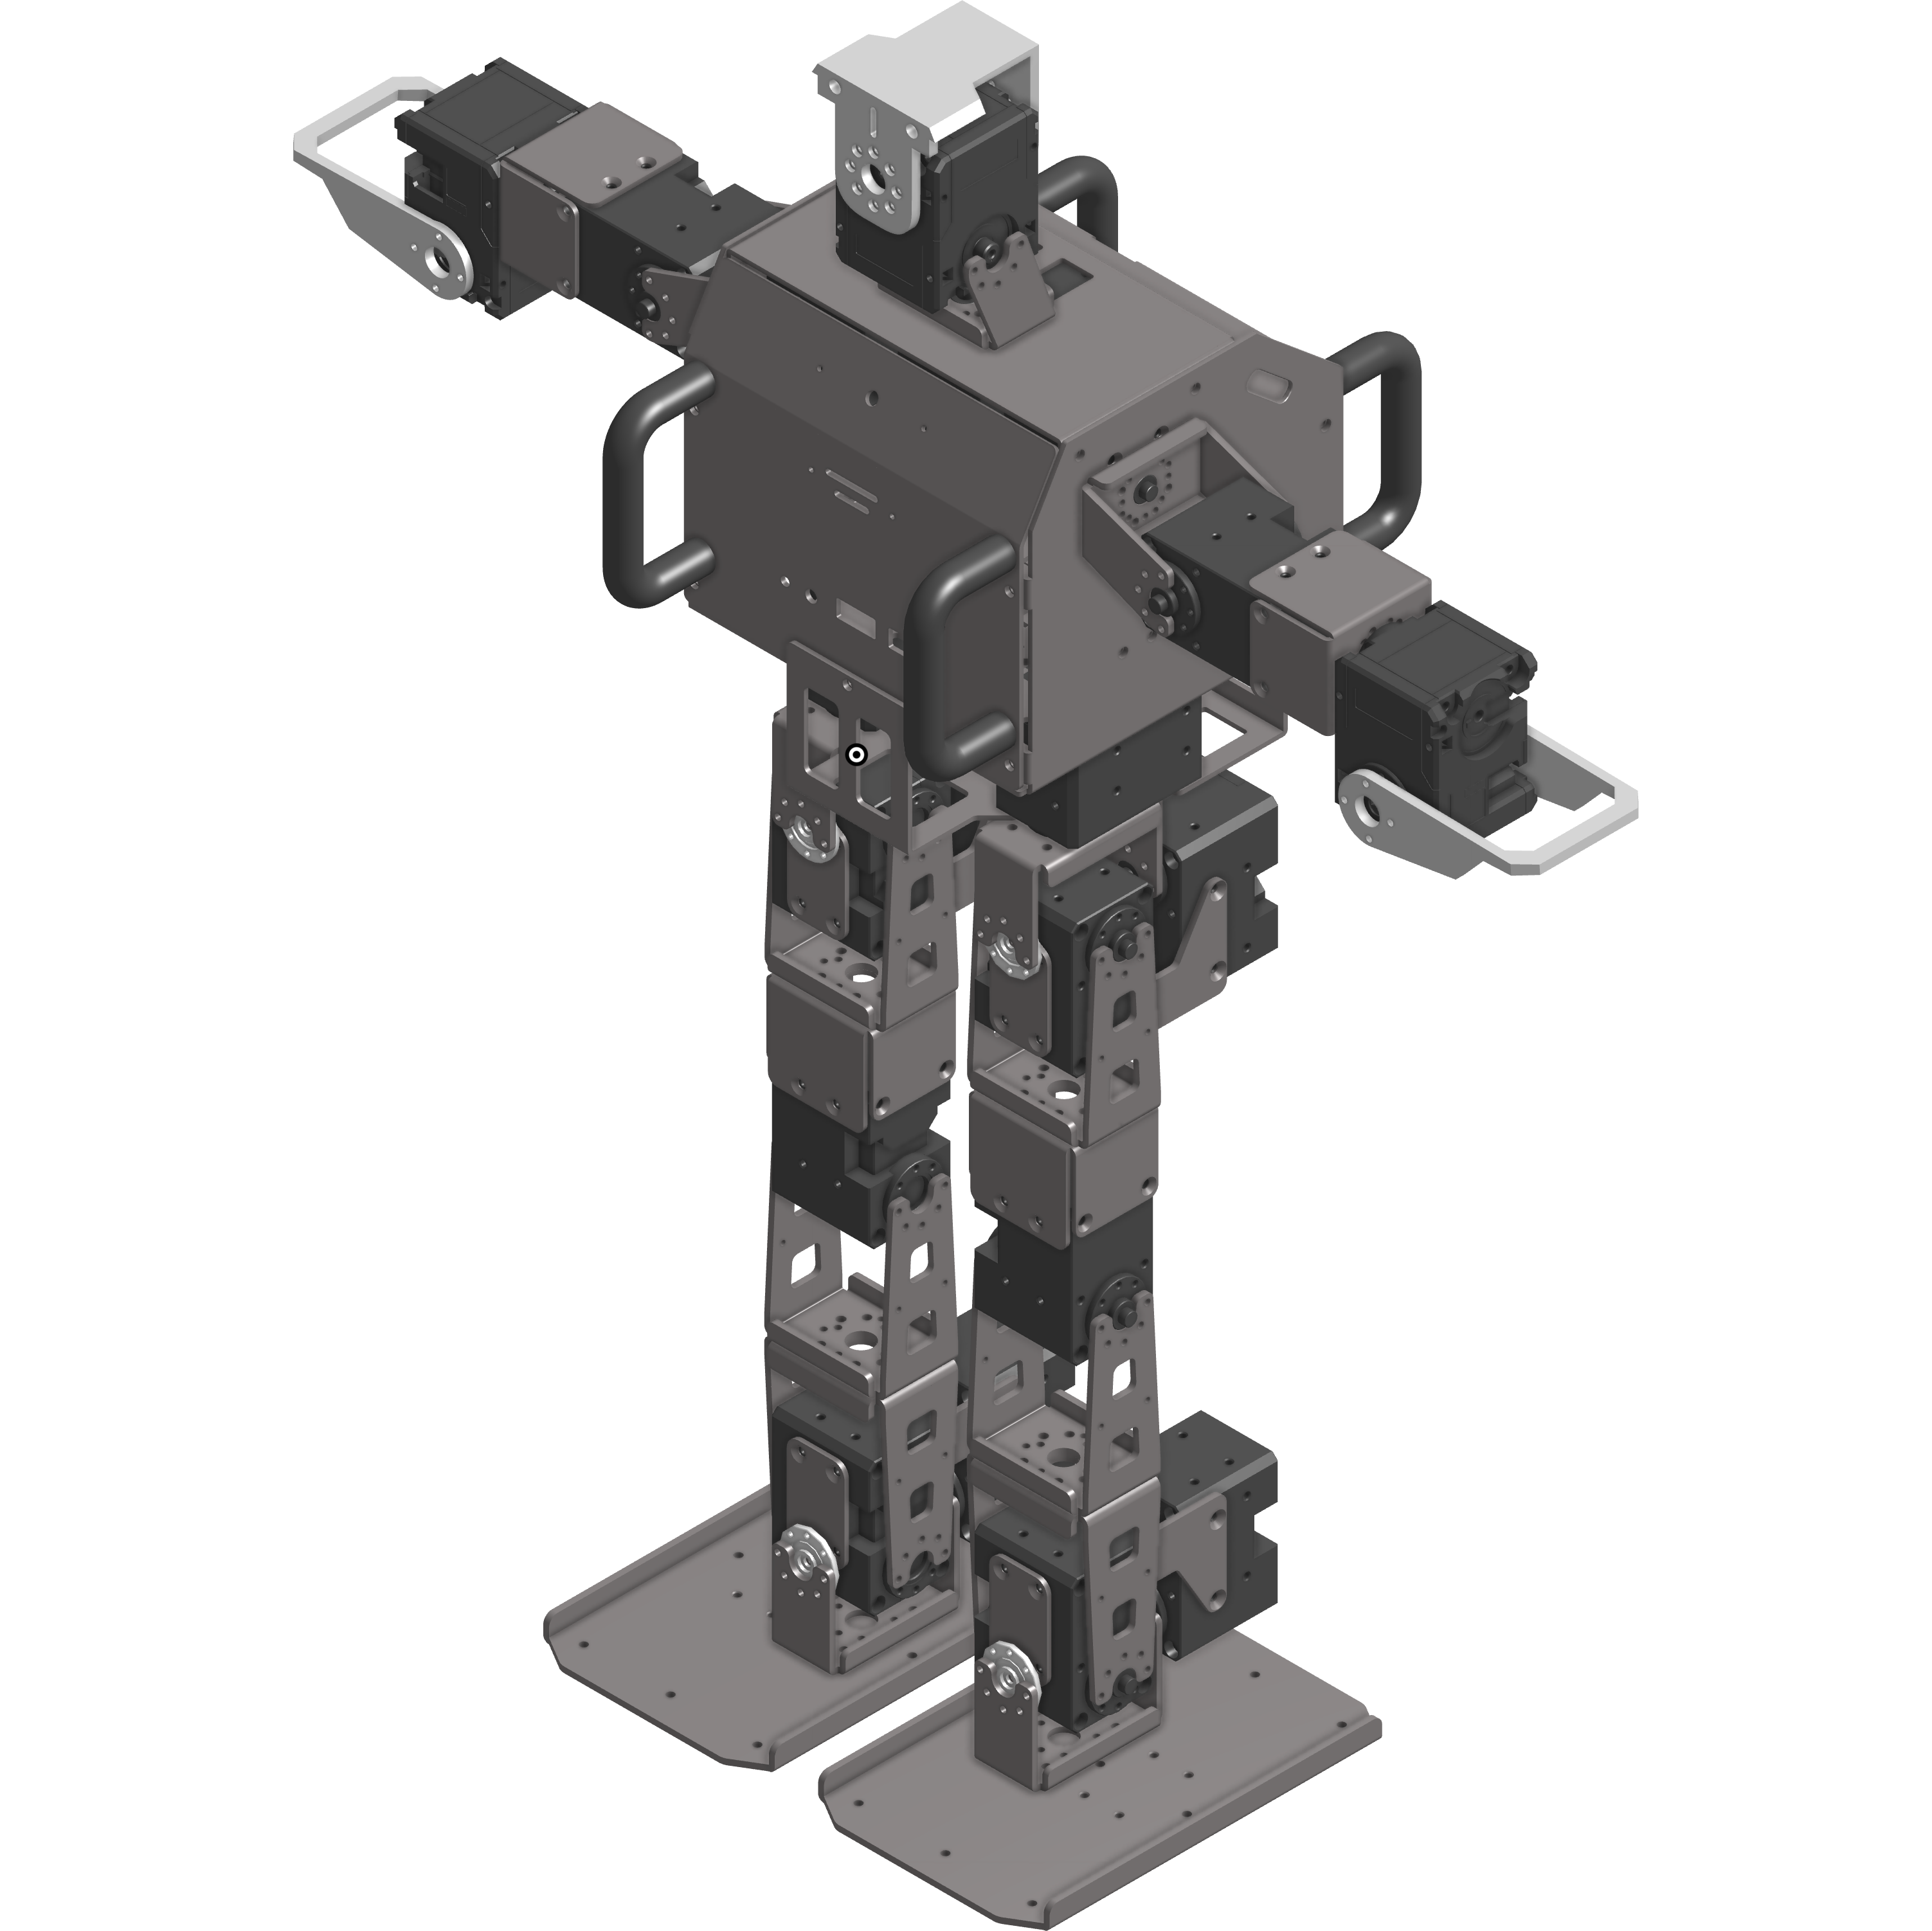
\includegraphics[width=\linewidth]{images/mod_robot1.png}
        \caption*{(a) Tampilan Robotis OP3 - Sisi Isometrik}
    \end{minipage}
    \hfill
    \begin{minipage}{0.48\textwidth}
        \centering
        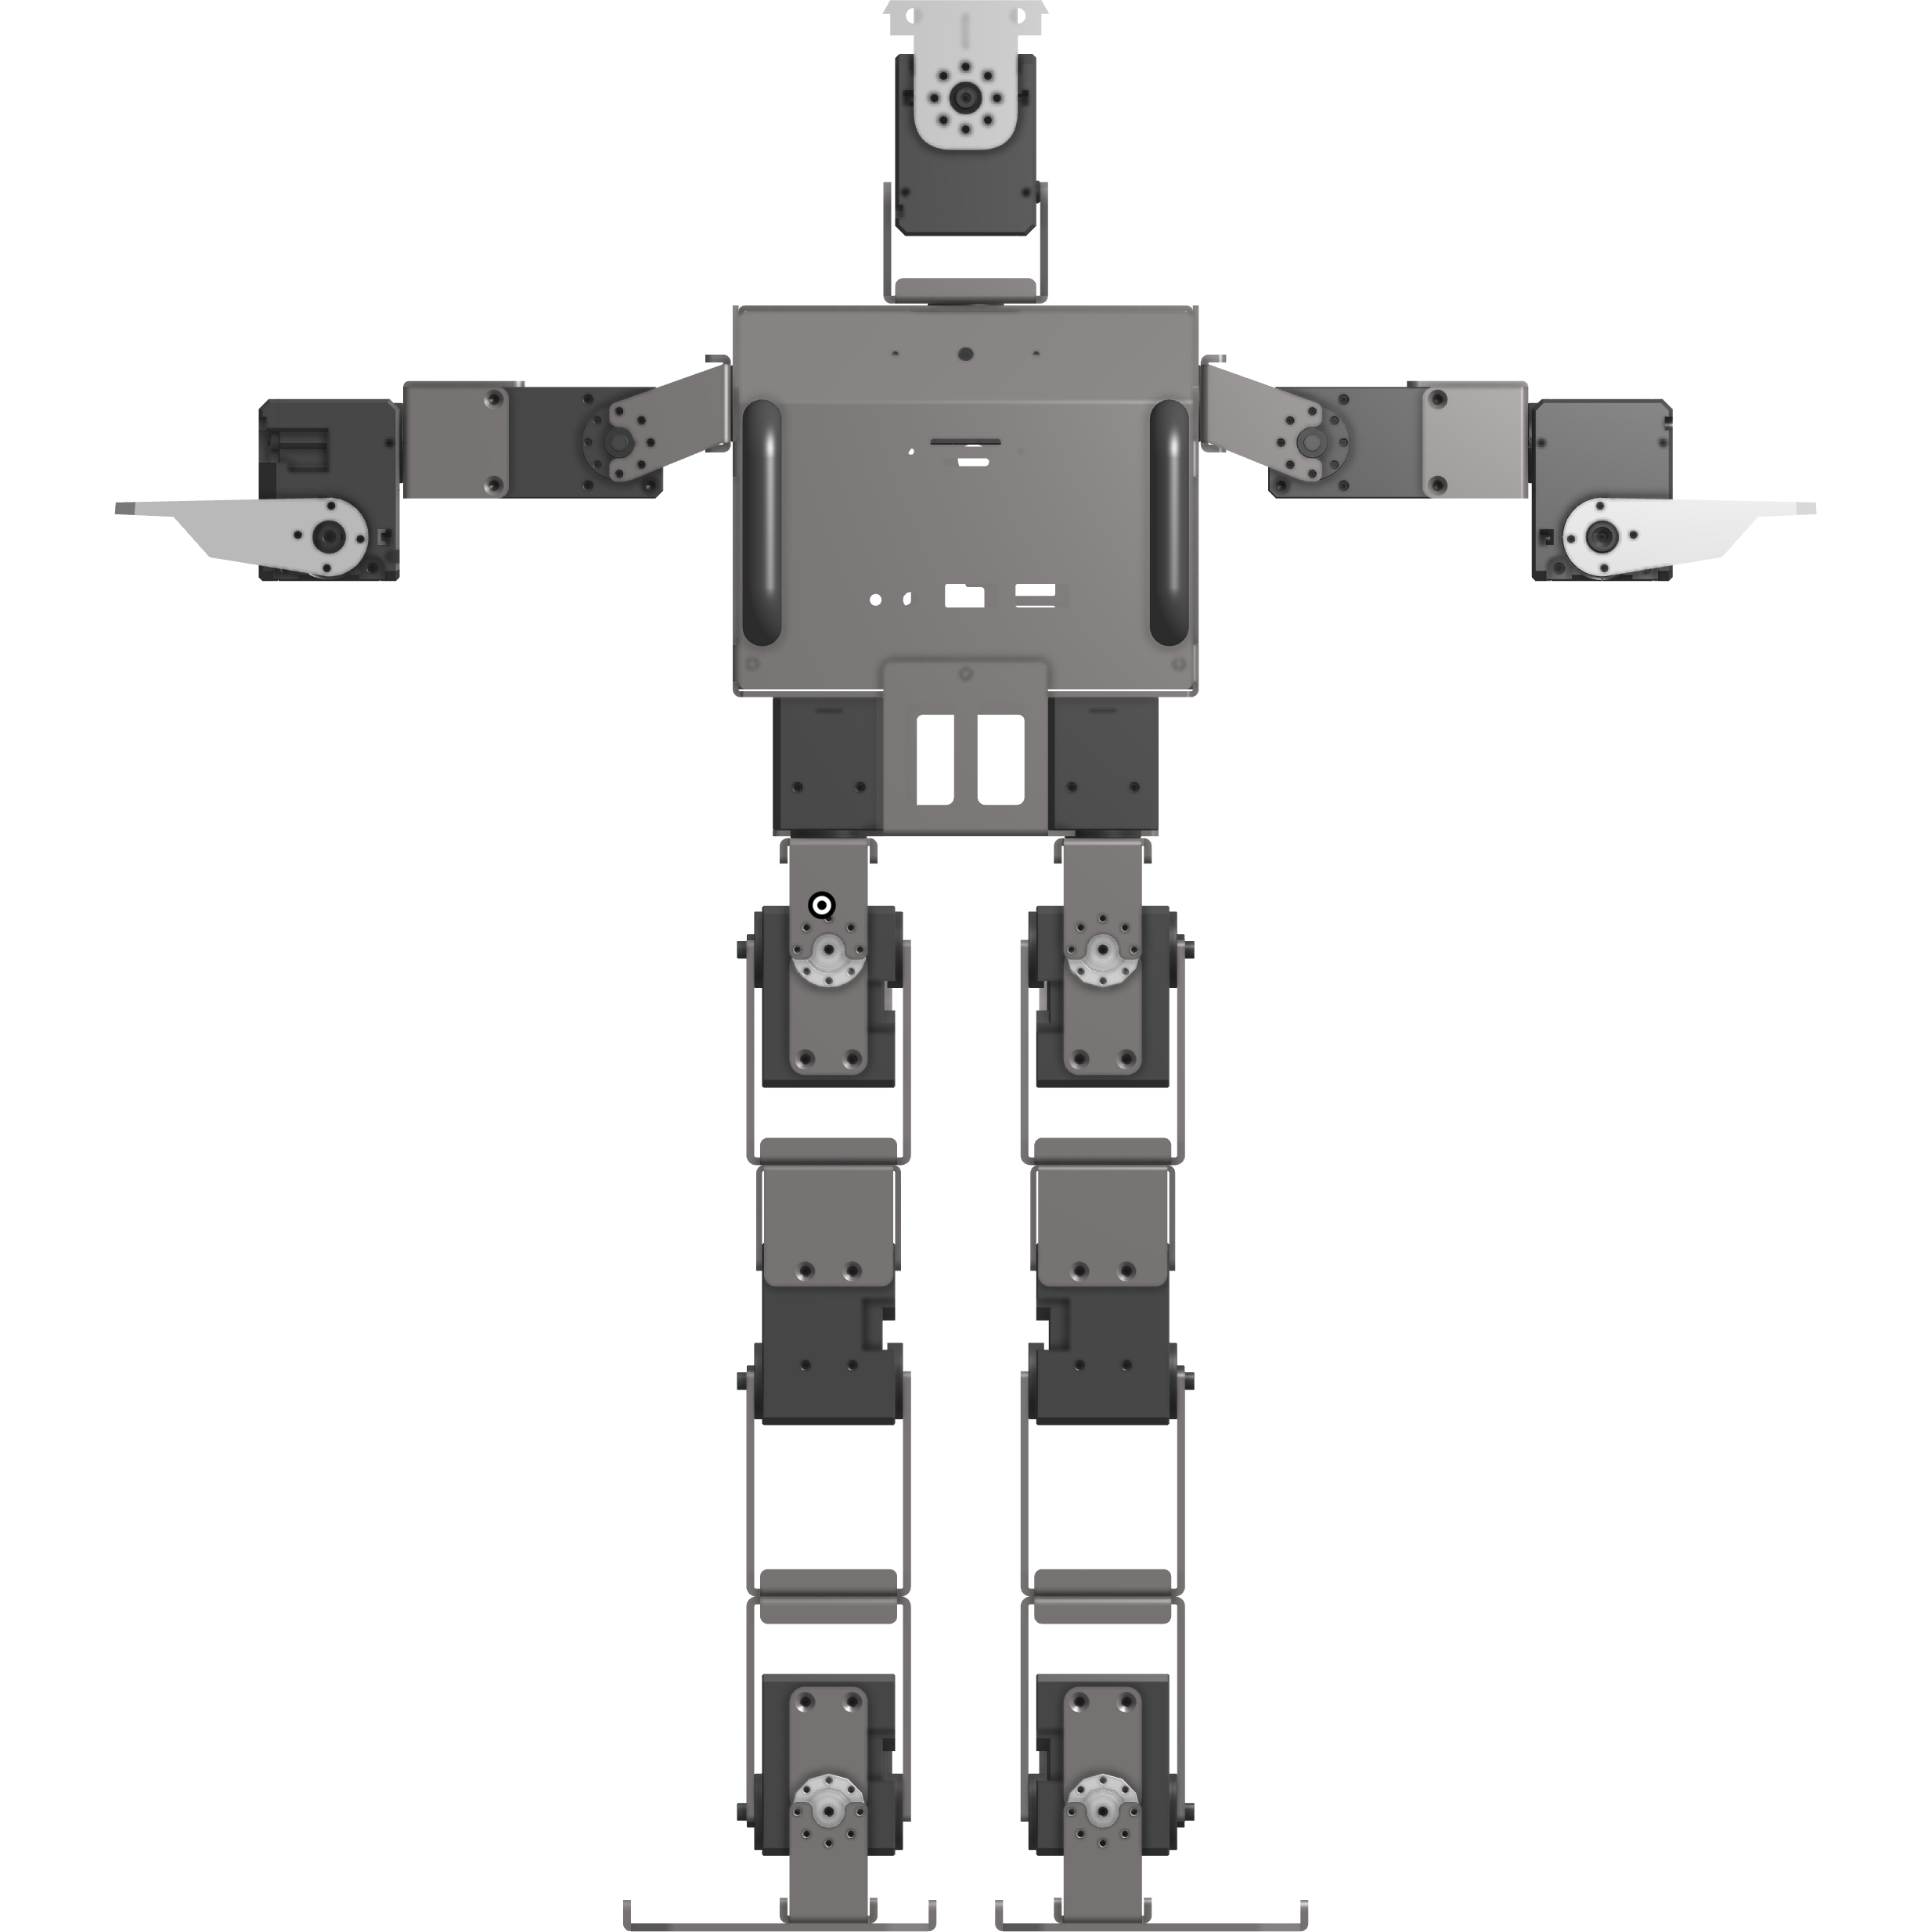
\includegraphics[width=\linewidth]{images/mod_robot2.png}
        \caption*{(b) Tampilan Robotis OP3 - Sisi Depan}
    \end{minipage}
    \caption{Tampilan fisik robot ROBOTIS-OP3 setelah modifikasi}
    \label{fig:modifikasi_fisik}
\end{figure}


Setelah pemasangan, dilakukan kalibrasi awal untuk memastikan sudut nol pada sumbu fleksi dan rotasi sesuai dengan orientasi default robot. Modifikasi fisik ini bertujuan agar robot mampu melakukan gerakan lengan yang lebih kompleks dan proporsional, sehingga mendukung representasi gerakan tari tradisional secara lebih realistis.

\subsection{Implementasi pada Robot}
\subsubsection{Transformasi Koordinat}

\begin{figure}[H]
    \centering
    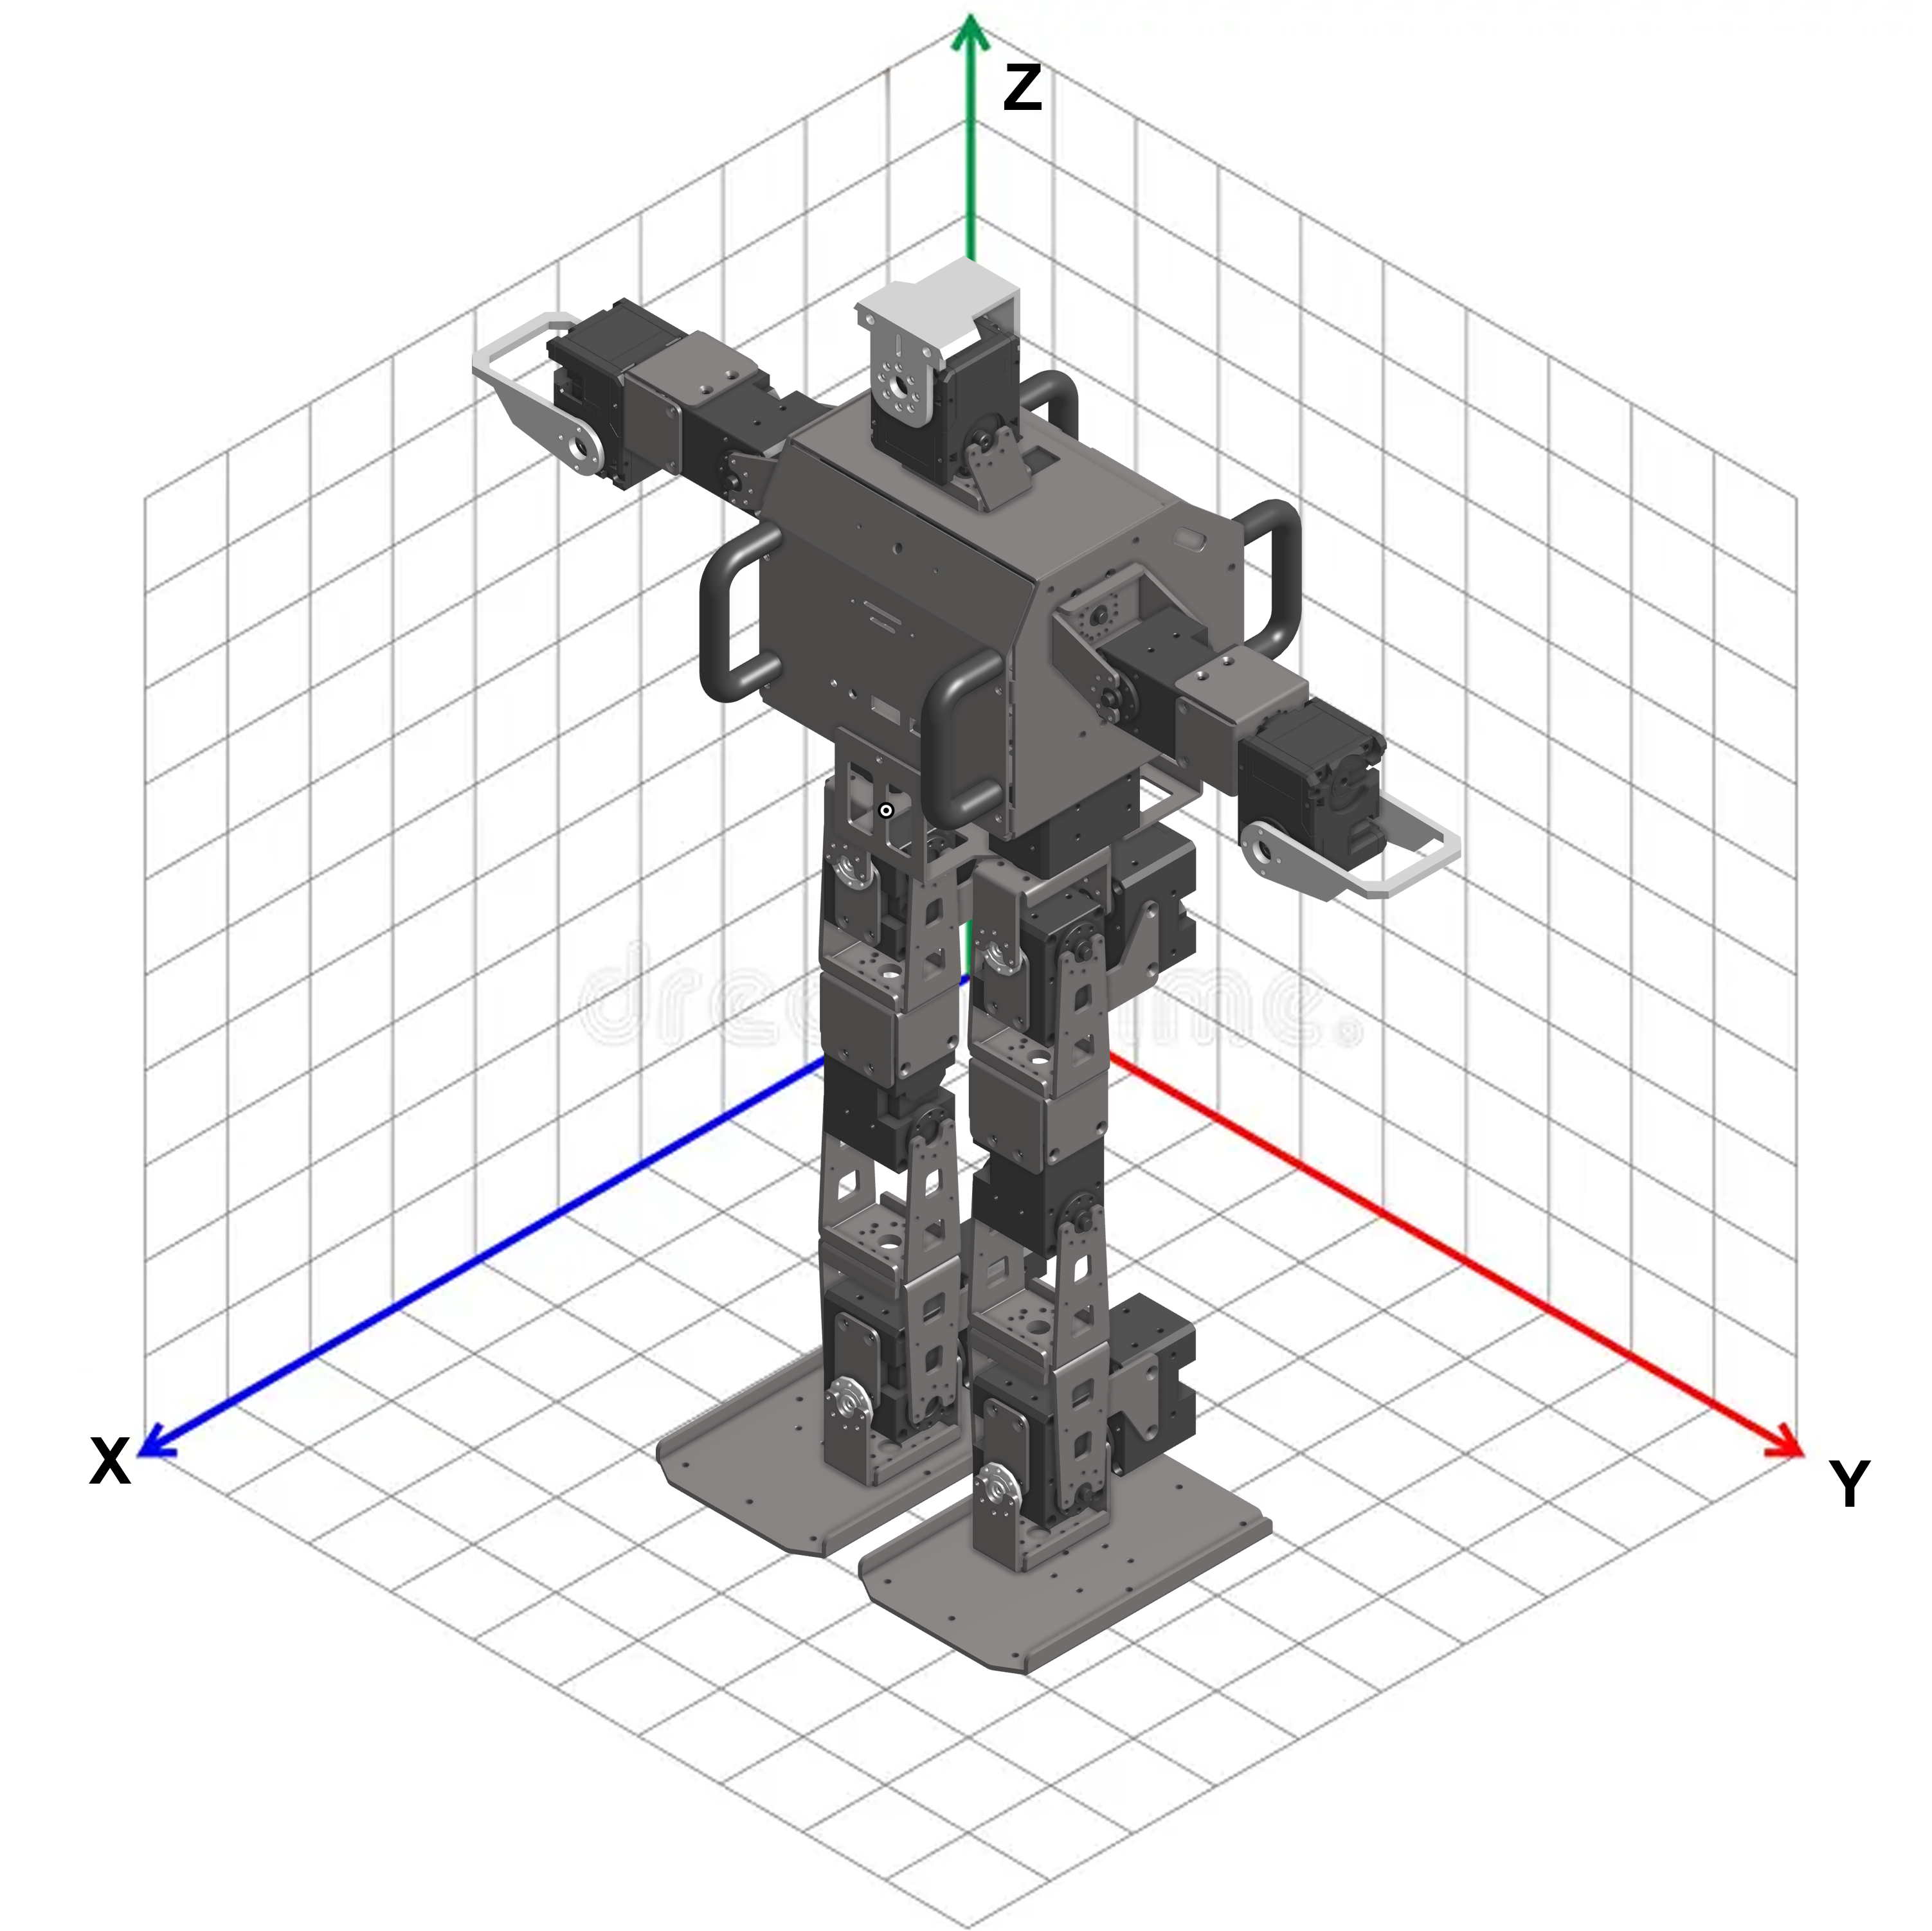
\includegraphics[width=0.6\textwidth]{images/mod_robot_coordinate.png}
    \caption{Visualisasi sistem koordinat robot}
    \label{fig:sistem_koordinat_robot}
\end{figure}

Karena terdapat perbedaan struktur mekanik, panjang sambungan, jumlah derajat kebebasan, serta sistem koordinat antara lengan manusia dan lengan robot ROBOTIS-OP3, maka koordinat 3D hasil estimasi pose tidak dapat langsung diterapkan secara langsung ke sistem kontrol robot. Untuk itu, diperlukan proses transformasi koordinat agar data pose manusia dapat diadaptasikan ke dalam sistem koordinat robot.

Transformasi yang dilakukan pada penelitian ini tidak melibatkan perubahan skala atau translasi global, melainkan hanya penyesuaian orientasi sumbu agar sesuai dengan definisi sumbu pada robot ROBOTIS-OP3. Pada sistem koordinat hasil estimasi pose, orientasi sumbu mengikuti konvensi kamera dengan:

\begin{itemize}
    \item Sumbu X sebagai kiri-kanan,
    \item Sumbu Y sebagai atas-bawah,
    \item Sumbu Z sebagai depan-belakang.
\end{itemize}

Sedangkan pada sistem koordinat robot ROBOTIS-OP3, orientasi sumbu diubah menjadi:

\begin{itemize}
    \item Sumbu X menjadi maju-mundur,
    \item Sumbu Y menjadi kiri-kanan,
    \item Sumbu Z menjadi atas-bawah.
\end{itemize}

Proses transformasi dilakukan dengan menukar posisi sumbu sesuai kebutuhan agar sistem koordinat manusia dapat dipetakan dengan benar ke sistem koordinat robot.

Selain penyesuaian orientasi sumbu, transformasi juga dilakukan untuk memindahkan posisi skeleton pose ke titik referensi yang diketahui, yaitu pada pusat koordinat (0,0,0). Hal ini bertujuan untuk menghilangkan translasi global atau pergeseran posisi dari pose manusia, sehingga seluruh gerakan hanya dihitung relatif terhadap titik tengah yang berupa bahu. Dengan menjadikan skeleton berada di titik nol, sistem hanya memproses perubahan orientasi dan sudut pergerakan, tanpa mempengaruhi posisi absolut di ruang global. Hal ini sesuai dengan implementasi pada robot, di mana pergerakan dilakukan secara \textit{in-place} dengan robot tidak berpindah tempat, hanya menggerakkan lengan dan kepala.


Hubungan transformasi koordinat untuk memetakan titik-titik tubuh manusia ke sistem koordinat robot dirumuskan sebagai berikut:

\begin{equation}
J'_{i} = \mathbf{A} \cdot (J_{i} - J_{1}), \quad i = 1,2,3
\end{equation}

\begin{equation}
J'_{i} = \mathbf{A} \cdot (J_{i} - J_{4}), \quad i = 4,5,6
\end{equation}

\begin{equation}
J'_{i} = \mathbf{A} \cdot (J_{i} - J_{7}), \quad i = 7,8
\end{equation}

Dengan penjelasan sebagai berikut:

\begin{itemize}
    \item $J_i$ merupakan koordinat titik kunci tubuh manusia dalam sistem koordinat dunia, sedangkan $J'_i$ adalah koordinat hasil transformasi dalam sistem koordinat robot.
    \item Matriks $\mathbf{A}$ adalah matriks rotasi yang dibentuk berdasarkan bidang segitiga yang menghubungkan bahu kiri ($J_1$), bahu kanan ($J_4$), dan panggul sebagai referensi.
\end{itemize}

Adapun penomoran titik kunci tubuh adalah sebagai berikut:

\begin{itemize}
    \item $J_{1}, J_{2}, J_{3}$ : Titik pada {lengan kiri}, secara berurutan meliputi \textit{shoulder left}, \textit{elbow left}, dan \textit{wrist left}.
    \item $J_{4}, J_{5}, J_{6}$ : Titik pada {lengan kanan}, secara berurutan meliputi \textit{shoulder right}, \textit{elbow right}, dan \textit{wrist right}.
    \item $J_{7}, J_{8}$ : Titik pada {kepala}, secara berurutan meliputi \textit{neck}, \textit{head}.
\end{itemize}

Transformasi ini dilakukan untuk memastikan bahwa seluruh pergerakan tubuh manusia dapat dipetakan secara tepat ke dalam sistem koordinat robot, dengan mempertimbangkan perbedaan orientasi sumbu dan struktur anatomi antara manusia dan robot. Proses ini memungkinkan perhitungan sudut sendi dilakukan secara konsisten dan sesuai dengan konfigurasi kinematika robot.

Proses transformasi koordinat tidak hanya melibatkan pergeseran titik referensi, tetapi juga pembentukan matriks rotasi $A$ yang berfungsi untuk menyelaraskan orientasi tubuh manusia dengan sistem koordinat robot. Matriks ini dibentuk berdasarkan tiga vektor ortonormal yang merepresentasikan arah sumbu lokal tubuh manusia, yaitu arah kiri-kanan, depan-belakang, dan atas-bawah.

Pembuatan matriks $A$ dilakukan dengan langkah-langkah sebagai berikut:

\begin{enumerate}
    \item Hitung vektor sumbu $z$ sebagai arah tegak lurus tubuh dari panggul($J_{9}$) ke pertengahan bahu:
    
    \begin{equation}
    {z} = \frac{(J_1 + J_4)}{2} - J_9
    \end{equation}
    
    Normalisasi vektor $z$ menjadi vektor unit:
    
    \begin{equation}
    {z}_{\text{axis}} = \frac{{z}}{||{z}||}
    \end{equation}
    
    \item Hitung vektor sumbu $y$ sebagai vektor dari bahu kanan ke bahu kiri:
    
    \begin{equation}
    {y} = J_1 - J_4
    \end{equation}
    
    Normalisasi vektor $y$ menjadi vektor unit:
    
    \begin{equation}
    {y}_{\text{axis}} = \frac{{y}}{||{y}||}
    \end{equation}
    
    \item Hitung vektor sumbu $x$ sebagai hasil perkalian silang antara ${y}_{\text{axis}}$ dan ${z}_{\text{axis}}$:
    
    \begin{equation}
    {x}_{\text{axis}} = {y}_{\text{axis}} \times {z}_{\text{axis}}
    \end{equation}
    
    Normalisasi vektor $x$ menjadi vektor unit:
    
    \begin{equation}
    {x}_{\text{axis}} = \frac{{x}_{\text{axis}}}{||{x}_{\text{axis}}||}
    \end{equation}
    
    \item Lakukan re-orthogonalization pada ${y}_{\text{axis}}$ agar tetap tegak lurus terhadap ${z}_{\text{axis}}$ dan ${x}_{\text{axis}}$:
    
    \begin{equation}
    {y}_{\text{axis}} = {z}_{\text{axis}} \times {x}_{\text{axis}}
    \end{equation}
    
    Normalisasi kembali:
    
    \begin{equation}
    {y}_{\text{axis}} = \frac{{y}_{\text{axis}}}{||{y}_{\text{axis}}||}
    \end{equation}
    
    \item Susun ketiga vektor ortonormal menjadi matriks rotasi $A$ sebagai berikut:
    
    \begin{equation}
    \mathbf{A} =
    \begin{bmatrix}
    x_1 & y_1 & z_1 \\
    x_2 & y_2 & z_2 \\
    x_3 & y_3 & z_3 \\
    \end{bmatrix}
    \end{equation}
    
    di mana ${x}_{\text{axis}} = [x_1, x_2, x_3]^T$, ${y}_{\text{axis}} = [y_1, y_2, y_3]^T$, dan ${z}_{\text{axis}} = [z_1, z_2, z_3]^T$.
\end{enumerate}


Matriks $\mathbf{A}$ ini digunakan untuk mentransformasikan koordinat dari sistem global (kamera) ke sistem lokal tubuh yang telah disesuaikan dengan orientasi robot. Proses ini memastikan bahwa orientasi sumbu tubuh manusia selaras dengan sistem koordinat robot, sehingga perhitungan sudut sendi dapat dilakukan secara konsisten dan akurat.


\subsubsection{Konversi Pose 3D ke Sudut Sendi}

Setelah koordinat pose 3D diselaraskan ke dalam sistem koordinat robot, langkah selanjutnya adalah menghitung sudut-sudut sendi berdasarkan arah vektor lengan atas, lengan bawah dan kepala. Sudut yang dihitung mencakup dua sudut pada bahu (\textit{pitch} dan \textit{roll}), dua sudut pada siku (\textit{twist} dan \textit{flexion}), dan 3 sudut pada kepala (\textit{pan}, \textit{tilt}, \textit{roll}). Proses ini memanfaatkan fungsi trigonometri invers dan operasi aljabar vektor.

Vektor lengan atas dan lengan bawah dapat didefinisikan sebagai:

\begin{equation}
\vec{V}_{\text{up}} = J'_{\text{elbow}} - J'_{\text{shoulder}} = 
\begin{bmatrix}
v^{up}_x \\
v^{up}_y \\
v^{up}_z
\end{bmatrix}
\end{equation}

\begin{equation}
\vec{V}_{\text{low}} = J'_{\text{wrist}} - J'_{\text{elbow}} = 
\begin{bmatrix}
v^{low}_x \\
v^{low}_y \\
v^{low}_z
\end{bmatrix}
\end{equation}

Sudut \textit{Shoulder Pitch} pada lengan kiri dinotasikan sebagai $\theta_{\text{LSPitch}}$, dihitung menggunakan fungsi $\arctan2$ terhadap komponen $-x$ dan $-z$ dari vektor lengan atas. Penggunaan tanda negatif pada kedua komponen dilakukan untuk menyelaraskan arah rotasi dengan orientasi sumbu pada robot, sehingga pergerakan yang dihasilkan sesuai dengan konfigurasi servo pada lengan kiri. Rumus perhitungan $\theta_{\text{LSPitch}}$ adalah sebagai berikut:

\begin{equation}
\theta_{\text{LSPitch}} = \arctan2\left(-v^{up}_x, -v^{up}_z\right)
\end{equation}

Sudut \textit{Shoulder Roll} pada lengan kiri dinotasikan sebagai $\theta_{\text{LSRoll}}$. Perhitungan sudut ini digunakan untuk mengetahui seberapa jauh lengan kiri bergerak ke samping (ke atas atau ke bawah). Sudut dihitung menggunakan fungsi $\arctan2$ sebagai berikut:

\begin{equation}
\theta_{\text{LSRoll}} = \arctan2\left(\sqrt{(v^{up}_x)^2 + (v^{up}_z)^2}, v^{up}_y\right)
\end{equation}

Perhitungan sudut $\theta_{\text{LEYaw}}$ dan $\theta_{\text{LERoll}}$ memerlukan transformasi koordinat lanjutan, yaitu dari sistem koordinat bahu kiri ke sistem koordinat siku kiri. Transformasi ini diperlukan agar perhitungan sudut di siku dilakukan secara lokal terhadap orientasi lengan atas. Hal tersebut didapatkan dengan melakukan rotasi pada vektor lebgan bawah dengan dua matriks rotasi berurutan, yaitu matriks $R_y$ dan matriks $R_x$ untuk mengoreksi orientasi terhadap sudut $\theta_{\text{LSPitch}}$ dan $\theta_{\text{LSRoll}}$.

\begin{equation}
\vec{V}'_{\text{low}} = R_x \cdot R_y \cdot \vec{v}_{\text{low}}
\end{equation}

Transformasi ini menghasilkan vektor lengan bawah dalam kerangka koordinat baru yang telah disejajarkan dengan orientasi lengan atas, sehingga sudut $-\theta_{\text{LEYaw}}$ dan $-\theta_{\text{LERoll}}$ dapat dihitung dengan lebih akurat.

Matriks rotasi $R_y$ dan $R_x$ masing-masing dituliskan sebagai berikut:

\begin{equation}
R_y(-\theta_{\text{LSPitch}}) = 
\begin{bmatrix}
\cos(-\theta_{\text{LSPitch}}) & 0 & \sin(-\theta_{\text{LSPitch}}) \\
0 & 1 & 0 \\
-\sin(-\theta_{\text{LSPitch}}) & 0 & \cos(-\theta_{\text{LSPitch}})
\end{bmatrix}
\end{equation}

\begin{equation}
R_x(-\theta_{\text{LSRoll}}) = 
\begin{bmatrix}
1 & 0 & 0 \\
0 & \cos(-\theta_{\text{LSRoll}}) & \sin(-\theta_{\text{LSRoll}}) \\
0 & -\sin(-\theta_{\text{LSRoll}}) & \cos(-\theta_{\text{LSRoll}})
\end{bmatrix}
\end{equation}

Tanda negatif pada setiap sudut digunakan untuk menyesuaikan arah rotasi dari sistem koordinat manusia ke sistem koordinat robot, agar sesuai dengan pergerakan fisik servo pada ROBOTIS-OP3.

Sudut \textit{Elbow Twist} pada lengan kiri dinotasikan sebagai $\theta_{\text{LETwist}}$, dihitung dari komponen vektor lengan bawah hasil rotasi. Perhitungan dilakukan menggunakan fungsi $\arctan2$ sebagai berikut:

\begin{equation}
\theta_{\text{LETwist}} = \arctan2\left(v'^{low}_x,v'^{low}_z\right)
\end{equation}

Sedangkan sudut \textit{Elbow Flexion} pada lengan kiri dinotasikan sebagai $\theta_{\text{LEFlex}}$, dihitung berdasarkan sudut antara vektor lengan atas dan vektor lengan bawah dengan menggunakan rumus dot product sebagai berikut:

\begin{equation}
\theta_{\text{LEFlex}} = \arctan2\left(-\sqrt{(v'^{low}_x)^2 + (v'^{low}_z)^2},v'^{low}_y\right)
\end{equation}

Perhitungan ini digunakan untuk menentukan seberapa besar lengan bawah menekuk (\textit{flexion}) dan berputar (\textit{twist}) relatif terhadap lengan atas dalam kerangka lokal yang telah disejajarkan.

Implementasi dari proses ini dilakukan pada kode program dengan memanfaatkan operasi vektor sederhana, seperti perkalian silang, dot product, dan normalisasi, yang diikuti dengan fungsi trigonometri $\arctan2$ dan $\arccos$. Langkah ini memastikan sudut yang diperoleh sesuai dengan batas pergerakan fisik servo pada robot humanoid ROBOTIS-OP3.


\begin{lstlisting}[style=plainbox, caption={Implementasi perhitungan sudut sendi sesuai rumus}]
aup_L = J_elbow - J_shoulder
alow_L = J_wrist - J_elbow

LShoulderPitch = np.arctan2(-aup_L[0], -aup_L[2])  # (X, Z)
LShoulderRoll = np.arctan2(np.sqrt(aup_L[0]**2 + aup_L[2]**2),
                 aup_L[1]
                 )

Ry = np.array([
    [np.cos(-LShoulderPitch), 0, np.sin(-LShoulderPitch)],
    [0, 1, 0],
    [-np.sin(-LShoulderPitch), 0, np.cos(-LShoulderPitch)]
])

Rx = np.array([
    [1, 0, 0],
    [0, np.cos(-LShoulderRoll), np.sin(-LShoulderRoll)],
    [0, -np.sin(-LShoulderRoll),  np.cos(-LShoulderRoll)]
])
alow_L_prime = Rx @ Ry @ alow_L
LElbowPitch = np.arctan2(-alow_L_prime[0], -alow_L_prime[2])
LElbowRoll = np.arctan2(
    -np.sqrt(alow_L_prime[0]**2 + alow_L_prime[2]**2),
    alow_L_prime[1]
)

ElbowFlexion = -np.degrees(angle_between_vectors(auJ_L, alow_L))
\end{lstlisting}
Begitu juga dengan bagian kepala, untuk mendapatkan sudut orientasi kepala, pertama-tama didefinisikan vektor kepala sebagai selisih antara posisi titik kepala dan titik leher:

\begin{equation}
\vec{V}_{\text{head}} = J'_{\text{head}} - J'_{\text{neck}} = 
\begin{bmatrix}
v^{head}_x \\[3pt]
v^{head}_y \\[3pt]
v^{head}_z
\end{bmatrix}
\end{equation}

Sudut \textit{Head Pan} dinotasikan sebagai $\theta_{\text{HPan}}$, yang merepresentasikan rotasi mendatar kepala (gerakan menengok ke kiri dan kanan). Sudut ini dihitung menggunakan fungsi $\arctan2$ terhadap komponen $y$ dan $x$ dari vektor kepala:

\begin{equation}
\theta_{\text{HPan}} = \arctan2\left(v^{head}_y, v^{head}_x\right)
\end{equation}

Sudut \textit{Head Roll} dinotasikan sebagai $\theta_{\text{HRoll}}$, yang menunjukkan kemiringan kepala ke samping (memiringkan kepala kiri atau kanan). Perhitungan dilakukan dengan:

\begin{equation}
\theta_{\text{HRoll}} = -\arctan2\left(v^{head}_y, v^{head}_z\right)
\end{equation}

Sedangkan sudut \textit{Head Tilt} atau \textit{Head Pitch}, dinotasikan sebagai $\theta_{\text{HTilt}}$, digunakan untuk mendeskripsikan gerakan kepala mendongak atau menunduk. Perhitungan dilakukan sebagai berikut:

\begin{equation}
\theta_{\text{HTilt}} = \arctan2\left(v^{head}_x, v^{head}_z\right)
\end{equation}

Perhitungan ketiga sudut ini dilakukan dalam kerangka lokal tubuh yang telah disesuaikan dengan orientasi robot, sehingga pergerakan kepala yang dihasilkan dapat sesuai dengan arah rotasi servo pada bagian kepala ROBOTIS-OP3.

\begin{lstlisting}[style=plainbox, caption={Implementasi perhitungan sudut kepala}]
ahead = J_head - J_neck  # vektor kepala
HeadPan = (np.arctan2(ahead[1], ahead[0]))
HeadRoll = -(np.arctan2(ahead[1], ahead[2]))
HeadTilt = (np.arctan2(ahead[0], ahead[2]))
\end{lstlisting}
\subsection{Penyimpanan Gerakan dalam Format JSON}

Setelah seluruh sudut sendi berhasil dihitung untuk setiap frame pose 3D, data gerakan kemudian disimpan dalam format berkas {JSON}. Penyimpanan ini bertujuan untuk memudahkan proses pemutaran ulang gerakan pada robot, serta sebagai format pertukaran data yang sederhana dan mudah diakses. Pada tahap ini, setiap frame hasil konversi disusun dalam struktur data Python \textit{dictionary}, dengan penamaan kunci yang sesuai dengan nama sendi pada robot. Contoh pemetaan sudut sendi ke nama kunci JSON dapat dilihat berikut:

\begin{lstlisting}[style=plainbox, caption={Pemetaan hasil sudut ke format JSON}]
frame_result = {
    "r_sho_pitch": angles_R["ShoulderPitch"],
    "l_sho_pitch": angles_L["ShoulderPitch"],
    "r_sho_roll": angles_R["ShoulderRoll"],
    "l_sho_roll": angles_L["ShoulderRoll"],
    "r_el_pitch": angles_R["ElbowTwist"],
    "l_el_pitch": angles_L["ElbowTwist"],
    "r_el_roll": angles_R["ElbowFlexion"],
    "l_el_roll": angles_L["ElbowFlexion"],
    "head_pan": angles_head["HeadPan"],
    "head_pitch": angles_head["HeadTilt"],
    "head_roll": angles_head["HeadRoll"],
}

results[str(frame_idx)] = frame_result
\end{lstlisting}

Setelah seluruh frame diproses, data hasil konversi disimpan dalam berkas {JSON} menggunakan fungsi {json.dump()}. Berikut contoh kode penyimpanan:

\begin{lstlisting}[style=plainbox, caption={Penyimpanan hasil gerakan dalam file JSON}]
output_file = "/home/luthfai/Devel/skripsi/pose_angles2.json"
with open(output_file, "w") as f:
    json.dump(results, f, indent=2)
\end{lstlisting}

Format file {JSON} ini berisi daftar sudut sendi per frame dalam satuan derajat, yang kemudian dapat digunakan sebagai masukan untuk perintah gerakan pada robot humanoid ROBOTIS-OP3.
Contoh isi file JSON hasil penyimpanan dapat dilihat pada Potongan Data berikut:

\begin{lstlisting}[style=plainbox, caption={Contoh data sudut sendi dalam format JSON}]
{
  "0": {
    "r_sho_pitch": -7.799538951688305,
    "l_sho_pitch": -10.71019173677621,
    "r_sho_roll": -46.40881222111872,
    "l_sho_roll": 48.35393974799908,
    "r_el_pitch": 121.56508280420996,
    "l_el_pitch": -103.9285816547141,
    "r_el_roll": -32.71889721964388,
    "l_el_roll": -17.327496671902992,
    "head_pan": -15.129533767700195,
    "head_pitch": -2.2988436222076416,
    "head_roll": 1.3416086435317993
  },
}
\end{lstlisting}

Data ini menunjukkan sudut sendi dalam satuan derajat untuk frame ke-0 pose 3D, yang kemudian dapat diproses sebagai perintah gerakan robot.

\subsection{Eksekusi Gerakan pada Robot}

Tahap akhir dalam sistem ini adalah menjalankan pergerakan lengan robot berdasarkan data sudut sendi yang telah dikonversi dan disimpan dalam berkas JSON. Proses ini dilakukan dengan memuat data sudut untuk setiap frame, mengonversi sudut derajat menjadi nilai posisi servo Dynamixel, kemudian mengirimkan perintah posisi ke semua aktuator secara sinkron.

File JSON yang berisi urutan sudut sendi dibaca dan diurutkan berdasarkan nomor frame. Data sudut kemudian dikonversi menggunakan fungsi \textit{deg\_to\_dxl} untuk menghasilkan nilai posisi servo yang sesuai dengan protokol pengendalian Dynamixel. Hasil konversi disimpan dalam variabel \textit{joint\_trajectories} yang memuat data untuk seluruh frame.

Pada tahap playback, program melakukan iterasi melalui setiap frame. Nilai posisi servo dikirimkan ke aktuator menggunakan metode write4ByteTxRx() atau melalui mekanisme sinkronisasi paket (\textit{sync write}), sehingga semua sendi bergerak serempak sesuai dengan urutan gerakan yang diinginkan. Kecepatan eksekusi dapat diatur menggunakan fungsi sleep() untuk mengatur interval antar frame.

Contoh kode Python yang digunakan dalam proses eksekusi gerakan robot adalah sebagai berikut:

\begin{lstlisting}[style=plainbox, caption={Kode eksekusi playback gerakan pada robot humanoid}]
for frame_idx in range(len(angle_data)):
    for joint_name, joint_id in JOINTS.items():
        pos = joint_trajectories[joint_name][frame_idx]

        # Konversi posisi menjadi 4 byte
        param_goal_position = [
            DXL_LOBYTE(DXL_LOWORD(pos)),
            DXL_HIBYTE(DXL_LOWORD(pos)),
            DXL_LOBYTE(DXL_HIWORD(pos)),
            DXL_HIBYTE(DXL_HIWORD(pos))
        ]
        groupSyncWrite.addParam(joint_id, 
                                bytearray(param_goal_position)
                                )
    groupSyncWrite.txPacket()
    groupSyncWrite.clearParam()

    time.sleep(1.0 / 30.0)
\end{lstlisting}

Proses ini memastikan robot dapat mereplikasi urutan gerakan hasil estimasi pose secara konsisten dengan kecepatan yang telah ditentukan.



\section{Implementasi Website}

Website yang dikembangkan pada penelitian ini berfungsi sebagai antarmuka utama untuk memproses video gerakan tari, melakukan estimasi pose 3D, menyimpan hasil konversi sudut, serta mengirim perintah gerakan ke robot humanoid. Sistem website dikembangkan menggunakan framework Flask, sedangkan proses inferensi model pose estimation dijalankan secara terpisah menggunakan Uvicorn dan FastAPI. Pemisahan ini dilakukan karena lingkungan Python untuk model estimasi membutuhkan pustaka tambahan seperti TensorFlow dan Torch yang berbeda versi dengan dependensi Flask.

Saat aplikasi pertama kali dijalankan, pengguna akan diarahkan pada halaman utama yang menampilkan judul Video Pose Estimation di bagian atas. Di sisi kiri halaman terdapat area unggah video, dengan ikon upload berukuran besar sebagai pusat interaksi. Bagian ini memungkinkan pengguna memilih video gerakan tari tradisional yang akan diproses. Setelah file dipilih, nama video akan muncul pada area log di bagian kanan bawah halaman, sehingga pengguna dapat memastikan bahwa file berhasil dimuat. Tampilan awal antarmuka website dapat dilihat pada Gambar~\ref{fig:website_awal}.

\begin{figure}[H]
    \centering
    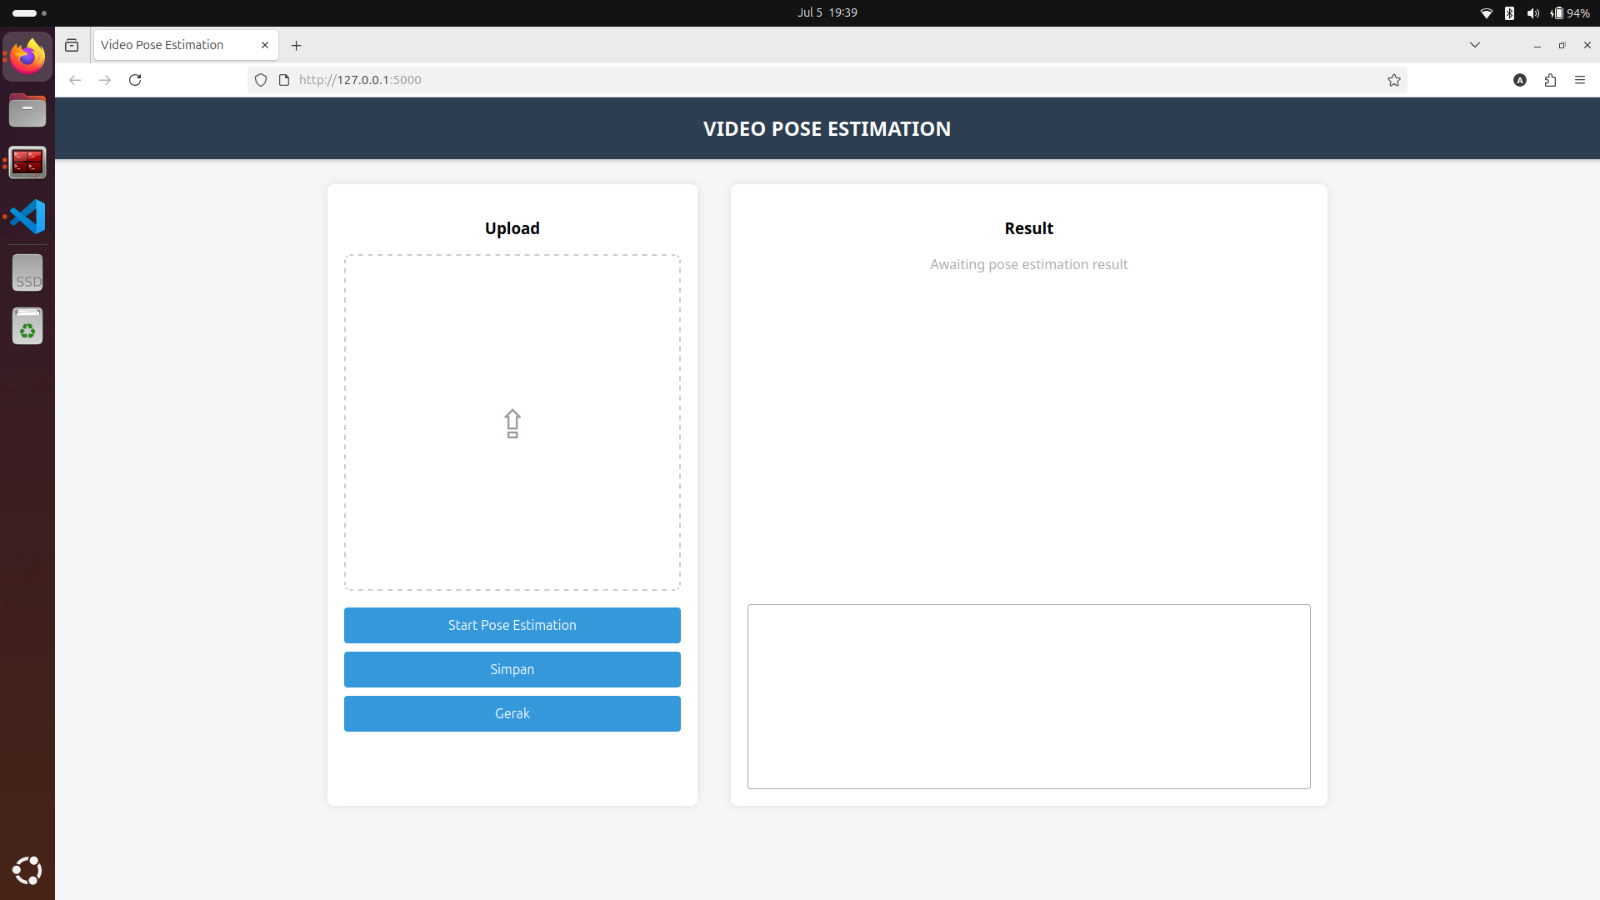
\includegraphics[width=0.9\textwidth]{images/tampilan1.jpeg}
    \caption{Tampilan awal website sebelum interaksi pengguna}
    \label{fig:website_awal}
\end{figure}

Pengguna dapat mengunggah video gerakan tari tradisional melalui tombol unggah. Setelah video dipilih, sistem akan menampilkan nama file pada area log. Contoh tampilan proses pemilihan video ditunjukkan pada Gambar~\ref{fig:upload_video}.

\begin{figure}[H]
    \centering
    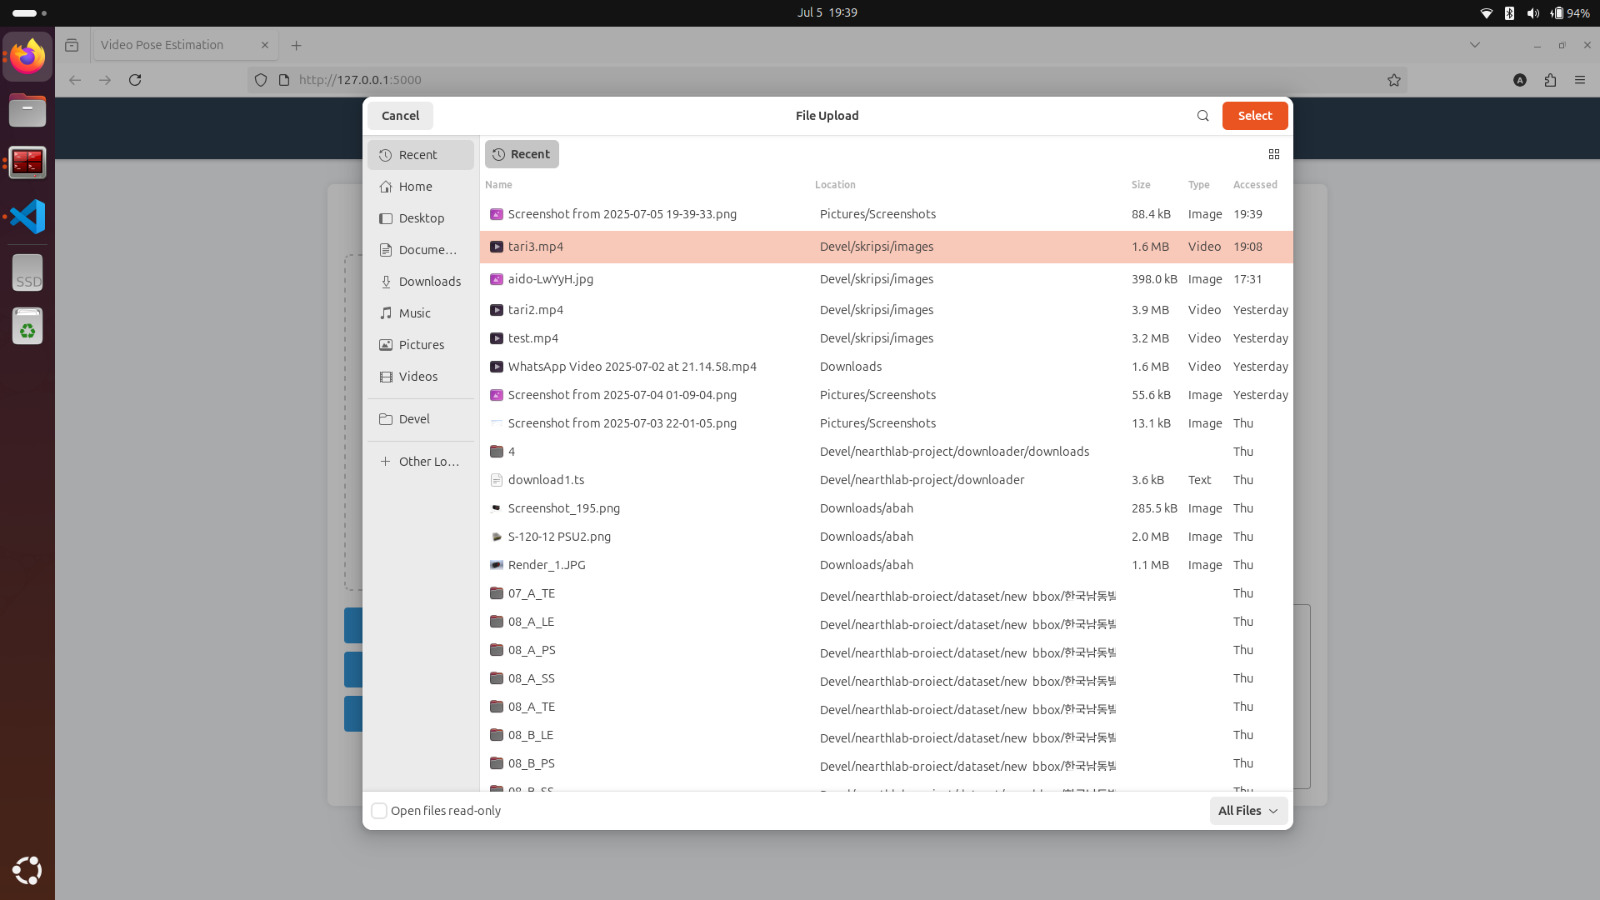
\includegraphics[width=0.9\textwidth]{images/tampilan2.jpeg}
    \caption{Proses upload dan pemilihan video}
    \label{fig:upload_video}
\end{figure}

Setelah video berhasil diunggah, pengguna dapat menekan tombol Start Pose Estimation yang terletak di bawah area unggah video. Ketika tombol ini ditekan, sistem akan melakukan proses estimasi pose 3D pada video secara bertahap. Proses ini dijalankan oleh server Uvicorn yang secara independen menangani komputasi model TensorFlow. Selama proses inferensi berlangsung, sistem menampilkan progress log dan visualisasi kerangka pose yang diperbarui secara real-time. Gambar~\ref{fig:proses_estimasi_pose} menunjukkan contoh tampilan proses estimasi pose.

\begin{figure}[H]
    \centering
    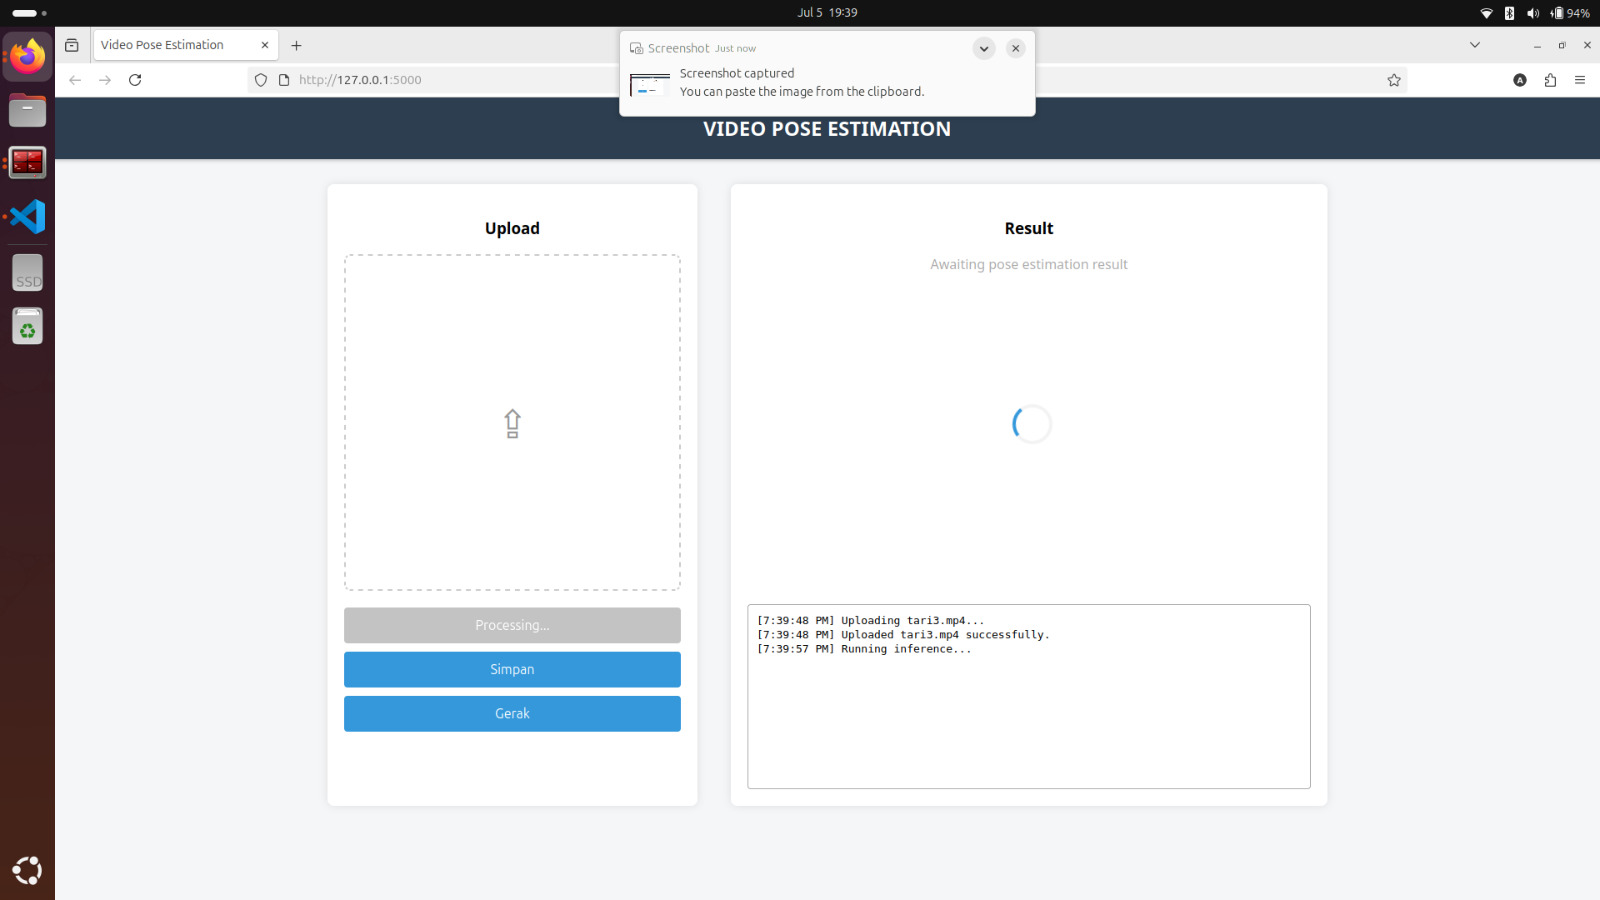
\includegraphics[width=0.9\textwidth]{images/tampilan4.jpeg}
    \caption{Tampilan proses estimasi pose 3D sedang berjalan}
    \label{fig:proses_estimasi_pose}
\end{figure}

Setelah estimasi selesai, hasil prediksi pose akan divisualisasikan dalam bentuk skeleton 3D pada sisi kanan halaman. Visualisasi ini dilengkapi keterangan frame saat ini dan total jumlah frame, sehingga pengguna dapat memantau hasil pose estimation secara lebih detail. Contoh hasil visualisasi ditunjukkan pada Gambar~\ref{fig:hasil_estimasi_pose}.

\begin{figure}[H]
    \centering
    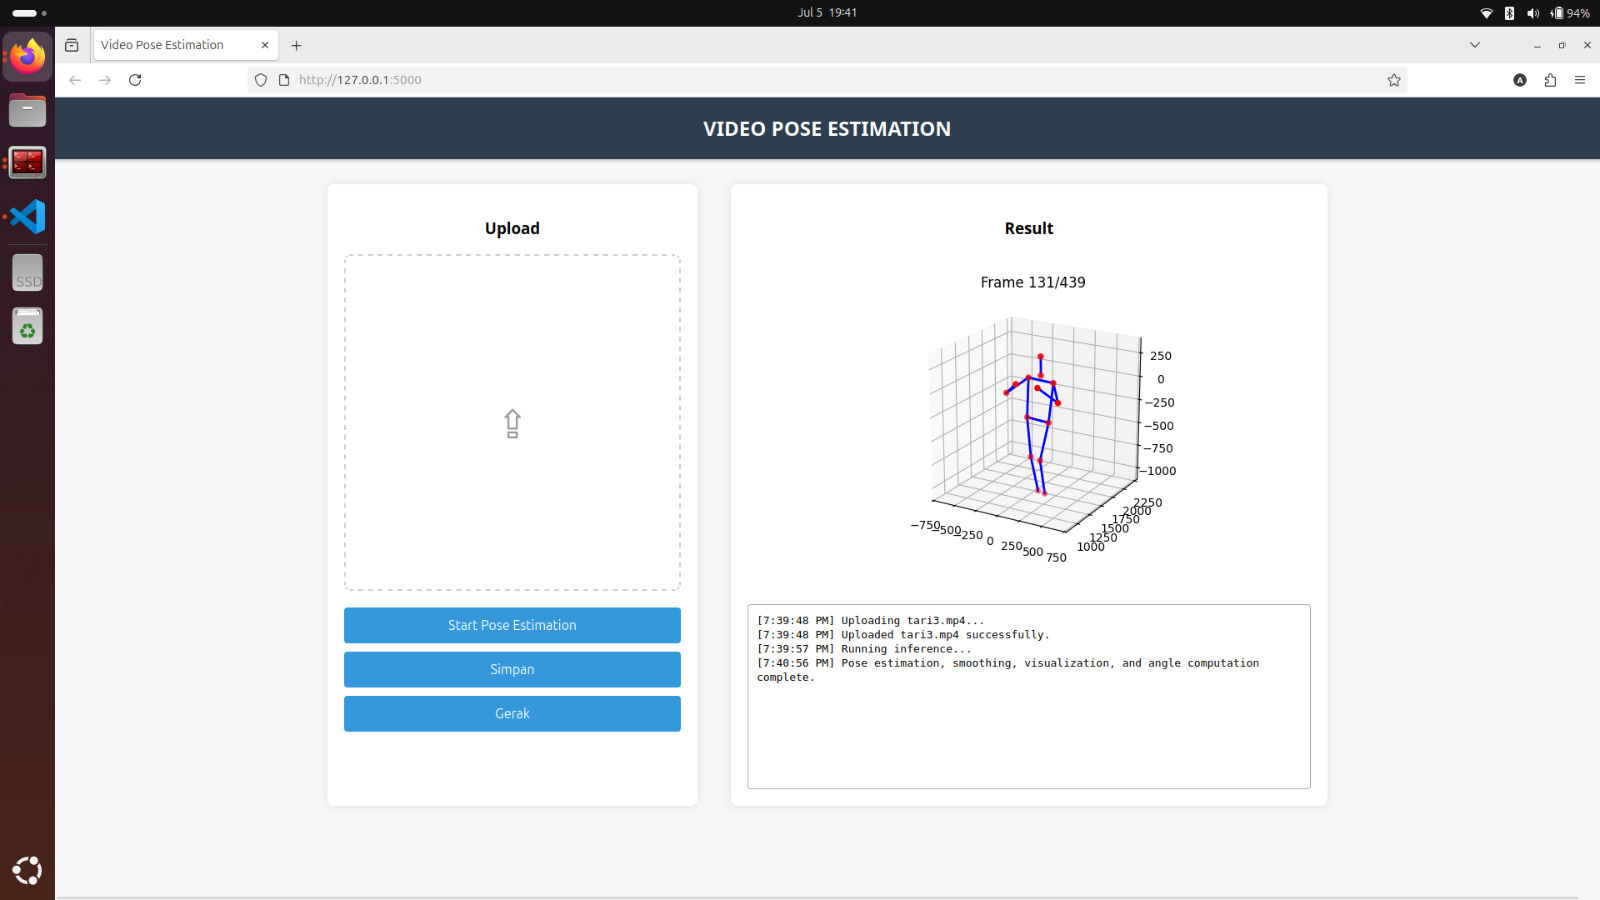
\includegraphics[width=0.9\textwidth]{images/tampilan5.jpeg}
    \caption{Hasil visualisasi pose 3D setelah proses estimasi selesai}
    \label{fig:hasil_estimasi_pose}
\end{figure}

Di bagian bawah area unggah video, terdapat tombol Simpan dan Gerak. Tombol Simpan digunakan untuk menyimpan hasil konversi sudut sendi dalam format JSON. File JSON yang dihasilkan berisi nilai sudut sendi untuk setiap frame, yang kemudian dapat digunakan sebagai input gerakan robot. Setelah penyimpanan selesai, sistem akan menampilkan notifikasi log yang menginformasikan direktori penyimpanan file. Contoh tampilan proses penyimpanan ditunjukkan pada Gambar~\ref{fig:simpan_pose}.

\begin{figure}[H]
    \centering
    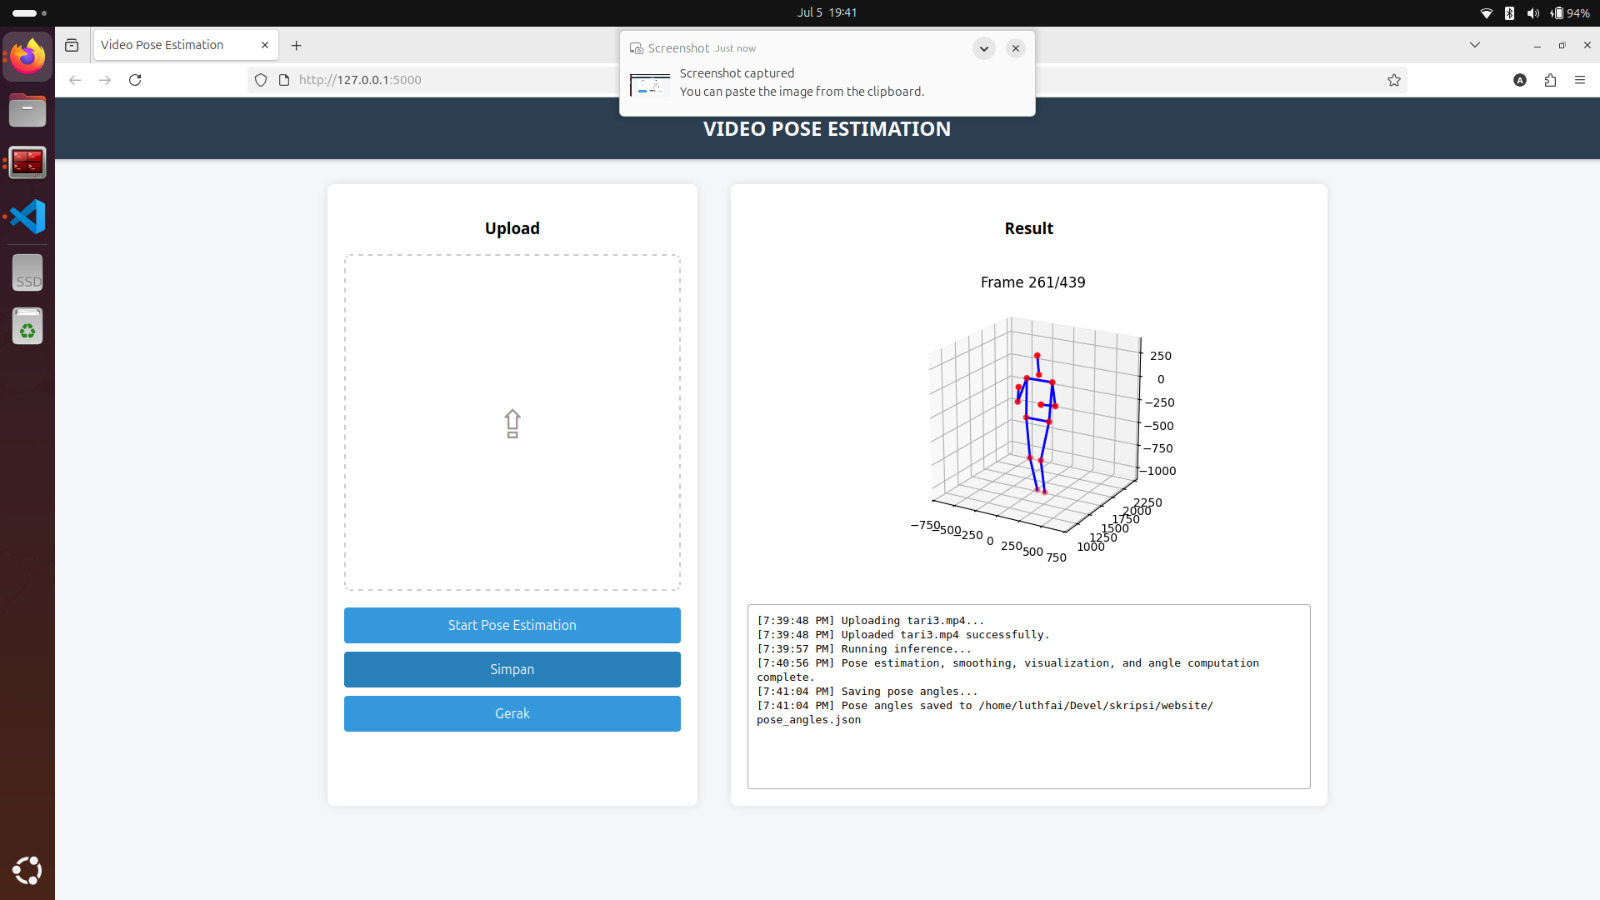
\includegraphics[width=0.9\textwidth]{images/tampilan6.jpeg}
    \caption{Tampilan saat proses penyimpanan data sudut sendi}
    \label{fig:simpan_pose}
\end{figure}

Tombol Gerak digunakan untuk memulai eksekusi playback gerakan pada robot humanoid ROBOTIS-OP3. Saat tombol ini ditekan, sistem akan membaca file JSON yang telah disimpan sebelumnya dan mengirimkan perintah posisi servo secara sinkron melalui protokol Dynamixel. Gambar~\ref{fig:gerakan_robot} menunjukkan tampilan antarmuka ketika proses gerakan robot dijalankan.

\begin{figure}[H]
    \centering
    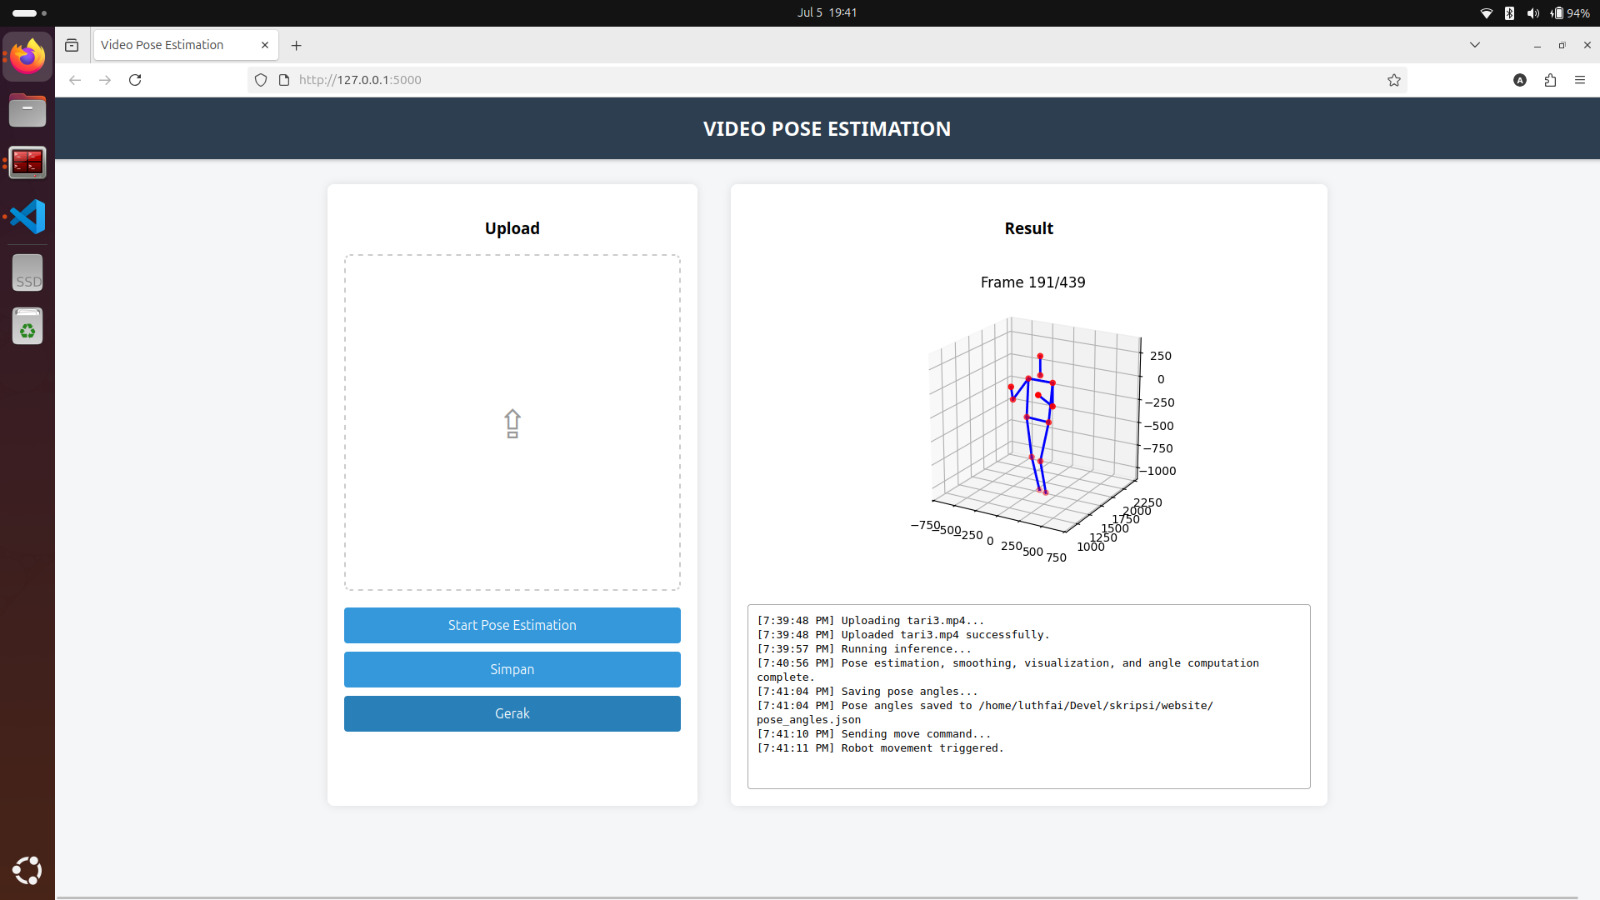
\includegraphics[width=0.9\textwidth]{images/tampilan7.jpeg}
    \caption{Tampilan saat proses playback gerakan robot berjalan}
    \label{fig:gerakan_robot}
\end{figure}

Dengan desain ini, seluruh proses mulai dari unggah video, estimasi pose, penyimpanan sudut sendi, hingga playback gerakan dapat dilakukan secara terpadu melalui satu antarmuka web yang sederhana namun lengkap. Pemisahan server Flask dan Uvicorn memungkinkan sistem berjalan lebih stabil karena proses komputasi model TensorFlow tidak memengaruhi kinerja web server utama.

\section{Pengujian Fungsional Sistem}

Pengujian fungsional dirancang untuk memastikan seluruh fitur utama pada sistem dapat berjalan sesuai dengan spesifikasi yang telah ditentukan. Metode pengujian menggunakan pendekatan \textit{black-box testing}, dengan skenario uji yang disusun berdasarkan masing-masing fitur yang terdapat pada sistem.

Pada tahap ini, pengujian fungsional aplikasi tidak dilakukan secara langsung oleh penulis, melainkan direncanakan untuk dieksekusi oleh anggota tim robotik yang bertugas mengelola implementasi pada perangkat robot. Pengujian ini mencakup alur penggunaan aplikasi, mulai dari input video hingga eksekusi gerakan pada robot ROBOTIS-OP3.

Tabel~\ref{tab:rencana_pengujian_fungsional} berikut menyajikan {rencana skenario pengujian fungsional} yang telah disusun.

\begin{longtable}{|c|p{2.5cm}|p{5cm}|p{4cm}|}
\caption{Rencana Pengujian Fungsional Sistem}
\label{tab:rencana_pengujian_fungsional} \\ \hline
\textbf{No} & \textbf{Fitur} & \textbf{Skenario Pengujian} & \textbf{Hasil yang Diharapkan} \\ \hline
\endfirsthead
\hline
\textbf{No} & \textbf{Fitur} & \textbf{Skenario Pengujian} & \textbf{Hasil yang Diharapkan} \\ \hline
\endhead

1 & Upload Video & Pengguna memilih dan mengunggah file video gerakan tari tradisional. & File berhasil diunggah dan nama file muncul di area log. \\ \hline
2 & Estimasi Pose dan Filtering & Pengguna menekan tombol \textit{Start Pose Estimation}. & Proses estimasi dan filtering berjalan hingga selesai tanpa error. \\ \hline
3 & Tampilan Estimasi Pose & Sistem menampilkan skeleton 3D hasil estimasi setiap frame. & Visualisasi skeleton muncul sesuai urutan frame video. \\ \hline
4 & Status Log & Sistem mencatat status proses pada area log. & Log status muncul pada setiap tahap proses. \\ \hline
5 & Penyimpanan Data & Pengguna menekan tombol \textit{Simpan} setelah estimasi pose selesai. & File JSON disimpan dalam direktori output. \\ \hline
6 & Playback Robot & Pengguna menekan tombol \textit{Gerak} untuk menjalankan robot. & Robot bergerak sesuai data sudut hasil estimasi pose. \\ \hline

\end{longtable}
